% ============================================================================
% P24 paper, SUBMISSION v7 (2026-11-23; user decision U-23a: body 4 pages, at most 5, references as needed,
% everything else summarized in the appendix, total at most 16 pages).  Built from main_v6_draft.tex
% (long version, kept unchanged as the full version).  The appendix is assembled from v6 sections by
% results/S5/paper_v7/assemble_v7.py and then edited by hand in main_v7.tex.
% Number sources: every paragraph or table row with numbers carries a "% src:" comment; the per-number ledger
% of v6 is results/S5/tn_ledger/ (all v7 numbers are copied from v6).
% Compile: tectonic -X compile --outdir build_v7 --keep-logs main_v7.tex (from paper/latex).
% ============================================================================
\documentclass[conference]{IEEEtran}

\IEEEoverridecommandlockouts

\usepackage{fontspec}  % 11-24: Times-like text font as in IEEE templates (TeX Gyre Termes)
\setmainfont{texgyretermes}[Extension=.otf, UprightFont=*-regular, BoldFont=*-bold, ItalicFont=*-italic, BoldItalicFont=*-bolditalic]
\usepackage{cite}
\usepackage{float}
\usepackage{amsmath,amssymb,amsfonts}
\usepackage{algorithmic}
\usepackage{graphicx}
\usepackage{textcomp}
\usepackage{xcolor}
\usepackage{array}
\usepackage{tabularx}
\usepackage{longtable}
\usepackage{wrapfig}
\usepackage{stfloats}
\usepackage[export]{adjustbox}
\usepackage{multirow}
\usepackage{booktabs}
\usepackage{pifont}
\usepackage{url}
\usepackage[letterpaper, top=1in, bottom=0.75in, left=0.75in, right=0.75in]{geometry}

% AUTO-GENERATED by `python -m p24.paper.build` -- do not edit by hand.
% One macro per number; sources, selectors and SHA16 are in numbers_manifest.csv.
\newcommand{\NBreakCaptureFiveTwelve}{43}
\newcommand{\NBreakCompileDiskFiveTwelve}{304}
\newcommand{\NBreakCompileEmptyFiveTwelve}{1826}
\newcommand{\NGenEvalCOneGOneCiHi}{+0.0037}
\newcommand{\NGenEvalCOneGOneCiLo}{$-$0.0037}
\newcommand{\NGenEvalCOneGOneDelta}{+0.0000}
\newcommand{\NGenEvalEZeroCiHi}{0.387}
\newcommand{\NGenEvalEZeroCiLo}{0.347}
\newcommand{\NGenEvalEZeroOverall}{0.367}
\newcommand{\NGenEvalPadDelta}{$-$0.0016}
\newcommand{\NHfourABestNameTenK}{B1}
\newcommand{\NHfourABestSecTenK}{1896}
\newcommand{\NHfourABootHiPctTenK}{4.5}
\newcommand{\NHfourABootLoPctTenK}{4.3}
\newcommand{\NHfourAGapPctTenK}{4.4}
\newcommand{\NHfourAOursSecTenK}{1979}
\newcommand{\NHfourASeedsHigherTenK}{10}
\newcommand{\NHfourAVerdictTenK}{refuted}
\newcommand{\NHfourBRatioTenK}{0.937}
\newcommand{\NHfourBVerdictTenK}{supported}
\newcommand{\NHfourCRatioTenK}{0.964}
\newcommand{\NHfourCVerdictTenK}{supported}
\newcommand{\NHfourSeedsTotal}{10}
\newcommand{\NMemCapGB}{20.0}
\newcommand{\NMemGraphBudgetGB}{6.4}
\newcommand{\NPoolGOneFiveTwelveBFourMB}{4696}
\newcommand{\NPoolGOneFiveTwelveBOneMB}{1172}
\newcommand{\NRealErrBOneWthreePct}{9.7}
\newcommand{\NRealErrBOneWtwoPct}{12.5}
\newcommand{\NRealErrOursWthreePct}{4.8}
\newcommand{\NRealErrOursWtwoPct}{8.8}
\newcommand{\NRealJudged}{13}
\newcommand{\NRealMaxErrPct}{12.5}
\newcommand{\NRealMemViolations}{6}
\newcommand{\NSTwoCostCOneFirstDiskS}{7.2}
\newcommand{\NSTwoCostCOneFirstEmptyS}{41.7}
\newcommand{\NSTwoCostCOneGOneSteadyMs}{72.1}
\newcommand{\NSTwoCostEZeroSteadyMs}{94.8}
\newcommand{\NSTwoRFiveTwelvePct}{4.7}
\newcommand{\NSTwoRMaxPct}{11.7}
\newcommand{\NSTwoShapes}{26}
\newcommand{\NTabAblBZeroWfiveSec}{2116}
\newcommand{\NTabAblBZeroWtwoSec}{2111}
\newcommand{\NTabAblLruWfiveSec}{2831}
\newcommand{\NTabAblLruWtwoSec}{2828}
\newcommand{\NTabAblNoPriorWfiveSec}{1996}
\newcommand{\NTabAblNoPriorWtwoSec}{1987}
\newcommand{\NTabAblOursWfiveSec}{1986}
\newcommand{\NTabAblOursWtwoSec}{1979}
\newcommand{\NTabAblThreeTiersWfiveSec}{2010}
\newcommand{\NTabAblThreeTiersWtwoSec}{2000}
\newcommand{\NTabAblVOneWfiveSec}{2032}
\newcommand{\NTabAblVOneWtwoSec}{2026}
\newcommand{\NTabIBreakCompileDiskFiveBFourCfg}{138}
\newcommand{\NTabIBreakCompileDiskFiveBOne}{304}
\newcommand{\NTabIBreakCompileDiskHiFiveBFourCfg}{141}
\newcommand{\NTabIBreakCompileDiskHiFiveBOne}{316}
\newcommand{\NTabIBreakCompileDiskHiSevenBOne}{206}
\newcommand{\NTabIBreakCompileDiskLoFiveBFourCfg}{134}
\newcommand{\NTabIBreakCompileDiskLoFiveBOne}{291}
\newcommand{\NTabIBreakCompileDiskLoSevenBOne}{177}
\newcommand{\NTabIBreakCompileDiskSevenBOne}{187}
\newcommand{\NTabIBreakCompileEmptyFiveBFourCfg}{718}
\newcommand{\NTabIBreakCompileEmptyFiveBOne}{1826}
\newcommand{\NTabIBreakCompileEmptyHiFiveBFourCfg}{725}
\newcommand{\NTabIBreakCompileEmptyHiFiveBOne}{1938}
\newcommand{\NTabIBreakCompileEmptyHiSevenBOne}{1087}
\newcommand{\NTabIBreakCompileEmptyLoFiveBFourCfg}{711}
\newcommand{\NTabIBreakCompileEmptyLoFiveBOne}{1791}
\newcommand{\NTabIBreakCompileEmptyLoSevenBOne}{1041}
\newcommand{\NTabIBreakCompileEmptySevenBOne}{1070}
\newcommand{\NTabIBreakGraphFiveBFourCfg}{159}
\newcommand{\NTabIBreakGraphFiveBOne}{43}
\newcommand{\NTabIBreakGraphHiFiveBFourCfg}{170}
\newcommand{\NTabIBreakGraphHiFiveBOne}{48}
\newcommand{\NTabIBreakGraphHiSevenBOne}{160}
\newcommand{\NTabIBreakGraphLoFiveBFourCfg}{143}
\newcommand{\NTabIBreakGraphLoFiveBOne}{39}
\newcommand{\NTabIBreakGraphLoSevenBOne}{88}
\newcommand{\NTabIBreakGraphSevenBOne}{95}
\newcommand{\NTabICompileDiskFiveBFourCfg}{7.4}
\newcommand{\NTabICompileDiskFiveBOne}{6.7}
\newcommand{\NTabICompileDiskSevenBOne}{6.9}
\newcommand{\NTabICompileEmptyFiveBFourCfg}{41.5}
\newcommand{\NTabICompileEmptyFiveBOne}{41.3}
\newcommand{\NTabICompileEmptySevenBOne}{41.8}
\newcommand{\NTabIFirstCOneGOneDiskFiveBFourCfg}{8.4}
\newcommand{\NTabIFirstCOneGOneDiskFiveBOne}{7.1}
\newcommand{\NTabIFirstCOneGOneDiskSevenBOne}{7.8}
\newcommand{\NTabIFirstCOneGOneEmptyFiveBFourCfg}{42.9}
\newcommand{\NTabIFirstCOneGOneEmptyFiveBOne}{41.7}
\newcommand{\NTabIFirstCOneGOneEmptySevenBOne}{42.6}
\newcommand{\NTabIFirstEZeroFiveBFourCfg}{0.7}
\newcommand{\NTabIFirstEZeroFiveBOne}{0.5}
\newcommand{\NTabIFirstEZeroSevenBOne}{0.6}
\newcommand{\NTabIPoolCOneGOneFiveBFourCfg}{2280}
\newcommand{\NTabIPoolCOneGOneFiveBOne}{628}
\newcommand{\NTabIPoolCOneGOneSevenBOne}{1278}
\newcommand{\NTabIPoolGOneFiveBFourCfg}{4726}
\newcommand{\NTabIPoolGOneFiveBOne}{1172}
\newcommand{\NTabIPoolGOneSevenBOne}{2566}
\newcommand{\NTabISteadyCOneGOneFiveBFourCfg}{344.1}
\newcommand{\NTabISteadyCOneGOneFiveBOne}{72.1}
\newcommand{\NTabISteadyCOneGOneSevenBOne}{166.5}
\newcommand{\NTabISteadyEZeroFiveBFourCfg}{402.9}
\newcommand{\NTabISteadyEZeroFiveBOne}{94.8}
\newcommand{\NTabISteadyEZeroSevenBOne}{205.9}
\newcommand{\NTabTightBOneWthreeSec}{3079}
\newcommand{\NTabTightBOneWtwoSec}{1896}
\newcommand{\NTabTightBZeroWthreeSec}{3437}
\newcommand{\NTabTightBZeroWtwoSec}{2111}
\newcommand{\NTabTightBudgetGB}{2.2}
\newcommand{\NTabTightOursWthreeSec}{3222}
\newcommand{\NTabTightOursWtwoSec}{1984}
\newcommand{\NTabWoneBOneTenK}{0.804}
\newcommand{\NTabWoneBSevenTenK}{0.768}
\newcommand{\NTabWoneOursTenK}{0.776}
\newcommand{\NTabWthreeBOneTenK}{0.896}
\newcommand{\NTabWthreeBSevenTenK}{0.985}
\newcommand{\NTabWthreeOursTenK}{0.937}
\newcommand{\NTabWtwoBOneTenK}{0.898}
\newcommand{\NTabWtwoBSevenTenK}{0.936}
\newcommand{\NTabWtwoOursTenK}{0.937}


\setlength{\textfloatsep}{10pt plus 2pt minus 4pt}
\setlength{\floatsep}{8pt plus 2pt minus 2pt}
\newcommand{\cYes}{\ding{51}}
\newcommand{\cNo}{\ding{55}}
\newcommand{\cPart}{(\ding{51})}
\newcommand{\cUnk}{?}
\newcommand{\cNa}{--}
\newcommand{\rh}[1]{\rotatebox[origin=l]{90}{#1}}
\newcommand{\tn}[1]{#1}% number traced to its source (see "% src:" comments)
\newcolumntype{Y}{>{\raggedright\arraybackslash}X}
\newcolumntype{P}[1]{>{\raggedright\arraybackslash}p{#1}}

\begin{document}

\title{Compile Now, Wait, or Build Ahead? Amortizing torch.compile and CUDA Graphs Across Request Shapes in Few-Step Diffusion Serving}

\author{
Kunlin Yang\textsuperscript{1}, Ibrahim (Abe) M. Elfadel\textsuperscript{2}\thanks{Corresponding author: ibrahim.elfadel@ku.ac.ae} \\
\textsuperscript{1}Department of Computer Science, \textsuperscript{2}Department of Computer and Information Engineering \\
Khalifa University of Science and Technology, Abu Dhabi, 127788, United Arab Emirates
}

\maketitle

\begin{abstract}
% src: internal:INT-01 (docs/internal_sources.md); results/S4X/x10/verdict/verdict_X10.json; internal:INT-02 (docs/internal_sources.md); results/S4P/p5d/verdict/d123_verdict.json; results/S4X/x9/verdict/h123_verdict.json; internal:INT-03 (docs/internal_sources.md); results/S4X/x8/verdict/h12_verdict.json
\noindent Few-step diffusion requests are so short (about 0.1~s at $512^2$) that launch overhead and the one-time costs of \texttt{torch.compile} and CUDA Graph capture rival the useful work, while real streams mix resolutions, batch sizes and guidance modes. For Stable Diffusion~1.5 with LCM-LoRA (fp16, four steps) on one RTX 4090, charging every one-time cost to service time and judging every claim against a line fixed before the data, we find: (1)~compilation is faster because it removes small kernels (cuDNN layout conversion alone equals \tn{81\%} of the net kernel-time reduction at $512^2$, large operators change by \tn{0.4\%}), and capture saves about the GPU's idle gaps (\tn{4.7\%} at $512^2$, \tn{0.55\%} at the largest shape); both held on a second model. (2)~An online, reuse-aware, memory-budgeted shape cache does not beat compiling each shape on first sight: the pre-registered hypothesis is refuted (\NHfourAGapPctTenK\% slower in simulation at $10^4$ requests), and even an oracle could gain under \tn{1\%} there. (3)~Moving the one-time cost offline gives the largest real speed-up: ahead-of-time (AOT) packages on disk need \tn{0.890} of eager's total time at $10^3$ requests per process and \tn{0.845} at $10^4$, a bounded set of 15 of 32 packages matches the full set at half the build time, and an H200 replay reproduced the gain (\tn{0.760}); the offline build is excluded and pays only when shared by many processes. At $10^4$ requests online compilation also beats eager (\tn{0.902}; our policy \tn{0.942}); from empty caches our policy ties eager (\tn{0.997}) while compiling on first sight takes \tn{4.44}$\times$ as long. (4)~A whole-process memory cap changed outputs when it bound a cuDNN workspace; expandable segments kept them bit-identical at \tn{13.1--13.3}~GiB peaks (the cap was then never reached).
\end{abstract}
\begin{IEEEkeywords}
torch.compile, CUDA Graphs, AOTInductor, diffusion serving, shape-bucket cache, break-even analysis, pre-registration
\end{IEEEkeywords}

% =============================================================================
\section{Introduction}\label{m:intro}
Few-step diffusion models~\cite{lcm,lcmlora} need about four UNet evaluations per image, so a request takes roughly a tenth of a second (\NSTwoCostEZeroSteadyMs{} ms at $512^2$ on our RTX 4090) and Python launch overhead is visible. CUDA Graphs~\cite{gray2019} and \texttt{torch.compile}~\cite{ansel2024} remove much of it and are standard advice~\cite{hf_fp16,pt_blog}. But each new input shape needs its own compiled code and its own graph, each with a compile or capture time, and graphs hold device memory. Real streams mix resolutions, batch sizes and guidance modes, so shapes are many and unevenly reused: compilation and capture are per-shape \emph{investments} whose return depends on the future of the stream.

With model and numerics fixed, we ask: why, mechanistically, do compilation and capture make a short request faster? Can an online, reuse-aware, memory-budgeted policy with eager fallback lower the total service time of a mixed stream, cold starts included? If not, what does, and when? Every claim is tested against a decision line written before its data (Sec.~\ref{m:method}); Tab.~\ref{m:tab:tests} lists all real-hardware tests with their verdicts.

\textbf{Contributions.} (C1)~A cost table by component and cold-start tier with break-even counts, and a kernel-level mechanism for both optimizations, checked on a second model (Sec.~\ref{m:mech}). (C2)~A pre-registered test of an online policy with a \emph{negative} primary result, a ceiling showing that even an oracle compile-or-eager selection could not have met its line, and four further online attempts, each failing for a measured reason (Sec.~\ref{m:online}). (C3)~Moving the one-time cost offline: AOT packages and a bounded bucket set chosen by the break-even model pass their lines on fresh real streams at $N{\ge}10^3$ (AOT missed its line at $N{=}300$), with a regime map of when each strategy wins (Sec.~\ref{m:offline}). (C4)~Credibility work: a simulator whose first validation failed and whose revision passed on new data, a memory cap whose bit-identity failure we traced to cuDNN, GenEval checks, a second platform and a failure catalogue (Secs.~\ref{m:mem}, \ref{m:trust}; App.~\ref{sec:failures}).

% src: results/S4P/p5d/verdict/d123_verdict.json; results/S4X/x9/verdict/h123_verdict.json
We claim no online policy faster than simple baselines. Real end-to-end gains over eager come from AOT with packages on disk and, at $N{=}10^4$ requests per process only, from online compilation; at $N{\le}10^3$ on multi-shape streams online policies at best tie eager. Code, data and one-command reproduction: \url{https://github.com/kleenY/p24-diffusion-compile-graphs}.

% =============================================================================
\section{Related Work and Position}\label{m:related}
PyTorch re-records a CUDA Graph per shape and advises padding to a few shapes~\cite{pt_cgtrees}; \texttt{torch.compile} recompiles on shape change, can run new shapes eagerly~\cite{pt_stance}, caches on disk, and AOTInductor builds packages ahead of time~\cite{pt_aoti}. LLM servers capture graphs for a static list of batch sizes and fall back to eager~\cite{vllm_cg,sglang_args}; PyGraph decides per graph whether capture pays and treats compile time as covered~\cite{pygraph}; Foundry materializes graphs offline to cut cold start~\cite{foundry}; Ekelund et al.\ model graph-creation overhead against replay benefit~\cite{ekelund2025}. Diffusion systems compile or capture at fixed resolutions~\cite{stablefast,onediff,fastusp,difflet} or batch mixed resolutions eagerly~\cite{patchedserve}; compile-or-eager is ski rental~\cite{karlin1988}. Within our non-exhaustive search, no work combines a multi-shape diffusion stream, a charge for every compile and capture cost, a graph-memory budget with admission and eviction, and eager fallback for rare shapes, validated on real replays. We claim no novelty for building ahead (an AOTInductor feature); we add the mechanism, the refutation and its ceiling, and the break-even selection of a bounded package set. App.~\ref{sec:related} and Tab.~\ref{tab:relwork} give the full comparison.

% =============================================================================
\section{Object, Protocol and Pre-Registration}\label{m:method}
% src: results/S2/equiv/equiv_matrix.csv; internal:INT-04 (docs/internal_sources.md)
\textbf{Object.} Stable Diffusion 1.5~\cite{rombach2022} with LCM-LoRA fused (hashed), fp16, four steps, guidance 1.0 (no CFG) or 1.5 (classifier-free guidance, CFG, doubles the UNet batch); one RTX 4090 (24~GB), PyTorch 2.9.1 (CUDA 12.6, cuDNN 9.10), Triton 3.5.1; memory in binary units. E0 is eager, G1 captures components in CUDA Graphs, C1 is \texttt{torch.compile} with static shapes, C1+G1 both; a shape is (height, width, batch, CFG). A configuration is accepted if its error against fp32 eager is at most twice E0's ($c{=}2$) and LPIPS to E0 at most 0.02: \tn{63} of 64 cells over 13 shape groups passed (graph padding at $512^2$ from batch 3 to 4 failed and is never used).

\textbf{Protocol.} The process is the statistical unit (bootstrap CIs); arms are interleaved; formal blocks run on an otherwise idle GPU with pinned cores and host load $\le$16. Cold tiers: \emph{empty} (compile caches cleared), \emph{disk} (caches on disk, new process), \emph{in-process}. Total service time counts every one-time cost.

\textbf{Workloads, policy, baselines.} Streams are declared from DiffusionDB~\cite{diffusiondb} prompts and resolutions (W1 one shape, W2 skewed, W3 uniform, W4 drifting, W5 cold burst; batch sizes and guidance modes from a declared distribution; prior and evaluation from disjoint halves). Our policy serves each shape in one of four modes (eager, G1, C1, C1+G1), upgrades a shape when accumulated would-be savings reach its upgrade cost (ski rental) or its prior reuse exceeds the break-even count, keeps graphs within a \NMemGraphBudgetGB{} GB budget with cost-aware eviction, and runs rare shapes and over-budget requests eagerly. Baselines: B0 eager, B1 compile on first sight, B2--B7 (dynamic shapes, reduce-overhead, PyTorch fallbacks, capture on first sight, LRU, static buckets, offline knapsack; App.~\ref{sec:method}); offline arms B1-AOT (packages for 32 prior shapes) and B1-AOT-K ($K$ packages). A trace-driven simulator composes measured costs and is validated on real replays.

\textbf{Pre-registration.} Every test had a card (hypothesis, metric, numeric line) made read-only before its deciding data; tuning used development seeds only; decisions used held-out seeds or fresh real streams; failures keep their original verdict, and a later fix is a new card (cards, timing and deviations: Apps.~\ref{app:cards}, \ref{app:dev}; all 36 attempts: App.~\ref{app:attempts}). Card labels index these appendices: X2/X2b memory cap, X5 and X9 replays at $N{=}10^4$, X8 empty caches, X10 second model; H4a--c and M1--M2 are hypotheses within a card; B1-R is B1 with the official tuning recipe.

\begin{table*}[t]
\caption{Pre-registered tests on real hardware and the primary simulator test (4090 unless marked; line fixed before the deciding data; verdicts as recorded). $N$ = requests per process; ratios are total service time. Simulator-only and exploratory attempts are listed in App.~\ref{app:attempts}.}
\label{m:tab:tests}
\centering\scriptsize
\setlength{\tabcolsep}{3pt}
\begin{tabularx}{\textwidth}{@{}P{3.6cm}P{3.6cm}YP{1.4cm}@{}}
\toprule
Test & Line & Result & Verdict\\
\midrule
% src: internal:INT-02 (docs/internal_sources.md)
H4a, policy vs.\ best online baseline (sim, W2, $10^4$) & $\ge$2\% faster on $\ge$8/10 seeds & \NHfourAGapPctTenK\% \emph{slower} than B1, 10/10 seeds & Refuted\\
% src: internal:INT-02 (docs/internal_sources.md); internal:INT-05 (docs/internal_sources.md)
Simulator v1 / v2 vs.\ real replays ($N{=}300$) & total-time error $\le$10\% & v1: up to \NRealMaxErrPct\% (all over-predicted); v2 (new seed): max \tn{2.26\%} & Fails / Holds\\
% src: internal:INT-06 (docs/internal_sources.md)
AOT, $N{=}300$ & AOT/B0 $\le$0.90 & \tn{0.985} (AOT/B1 \tn{0.423}) & Fails\\
% src: results/S4P/p5d/verdict/d123_verdict.json
AOT, $N{=}10^3$, 3 streams & $\le$0.90 combined & \tn{0.890} & Holds\\
% src: internal:INT-03 (docs/internal_sources.md)
Bounded set $K{=}15$, $N{=}10^3$ & $K$/full $\le$1.02; with build $\le$0.564 & \tn{0.994}/\tn{1.002}; \tn{0.514}/\tn{0.516} & Holds\\
% src: results/S4X/x5/verdict/e12_verdict.json
Policy vs.\ B1, $N{=}10^4$ (X5) & ordering as predicted; error $\le$10\% & policy/B1 \tn{1.045}; errors \tn{1.6/1.8\%} & Holds\\
% src: results/S4X/x9/verdict/h123_verdict.json
Eager and AOT arms, $N{=}10^4$ (X9) & B1/B0 $\le$0.95; policy/B0 $\le$0.98; AOT/B0 $\le$0.90 & \tn{0.902}; \tn{0.942}; \tn{0.845} & Holds\\
% src: results/S4X/x8/verdict/h12_verdict.json
Empty caches, $N{=}10^3$ (X8) & policy/B0 $\le$1.05; B1/B0 $\ge$2 & \tn{0.997}; \tn{4.44} & Holds\\
% src: internal:INT-06 (docs/internal_sources.md)
Official recipe + fix, $N{=}300$ & B1-R/B1 $\le$0.975 & \tn{1.088} [\tn{1.069}, \tn{1.114}] & Fails\\
% src: internal:INT-07 (docs/internal_sources.md)
Background compilation (GPU step) & eager slowdown $f\le$0.3 & $f{=}$\tn{8.6} & Fails\\
% src: internal:INT-03 (docs/internal_sources.md)
Whole-process cap 16~GiB (X2) & peak, no crash, bit-identical, time & bit-identity fails in 1 of 4 cells & Fails\\
% src: internal:INT-03 (docs/internal_sources.md)
Expandable segments + cap (X2b) & same lines & 4/4 cells; peaks \tn{13.1--13.3 GiB} & Holds\\
% src: internal:INT-02 (docs/internal_sources.md); results/S4/mem_43b/fit/verdict.json
Whole-process memory model refit & 13/13 cells conservative and within 1~GB & \tn{4} of 13 & Fails\\
% src: results/S4X/x4/analysis/geneval_S4X_X4_verdict.txt; internal:INT-03 (docs/internal_sources.md)
GenEval, $512^2$ (E0 vs.\ C1+G1, AOT, CFG) & $|\Delta|\le$0.02 & all within (largest $|\Delta|$ \tn{0.0006}) & Holds\\
% src: internal:INT-03 (docs/internal_sources.md)
H200: cost-model signs; AOT, $N{=}10^3$ & sign predictions; AOT/B0 $\le$0.90, error $\le$5\% & \tn{8/9}, \tn{14/14}; \tn{0.760}, \tn{1.9\%} & Holds\\
% src: internal:INT-03 (docs/internal_sources.md)
H200: node-local empty-cache rerun & first requests within $\pm$10\% of reference & \tn{0/24} failures, but \tn{19--25\%} faster & Fails\\
% src: results/S4X/x10/verdict/verdict_X10.json
Second model, SD-Turbo (X10) & mechanism lines M1, M2 & non-large \tn{99\%}; saving/idle \tn{1.19} & Holds\\
\bottomrule
\end{tabularx}
\end{table*}

% =============================================================================
\section{Why Compilation and Capture Are Faster}\label{m:mech}
% src: internal:INT-01 (docs/internal_sources.md); results/S4X/ceiling/kernel_breakdown.csv
We classified every kernel of steady-state requests in Nsight Systems traces (Tab.~\ref{m:tab:kernels}). At $512^2$ without CFG compilation cuts kernel time by \tn{20.7\%} (wall time \tn{20.3\%}); the large operators (convolution, GEMM, attention) change by \tn{0.4\%}. Removing cuDNN layout-conversion kernels (\texttt{nchwToNhwc} and back) alone saves an amount equal to \tn{81\%} of the net reduction; normalization and element-wise kernels are fused away while new Triton kernels are added back. Converting eager to \texttt{channels\_last} made it \tn{11--22\%} \emph{slower}, so here this gain is reachable only through compilation. Because large operators dominate bigger shapes (\tn{52.5\%} to \tn{67.5\%} of eager kernel time), the ceiling of compilation falls from \tn{42.7\%} at $256^2$ to \tn{32.4\%} at $768^2$ (batch four, CFG); measured savings are \tn{24.6\%} and \tn{8.7\%}.

\begin{table}[t]
\caption{GPU kernel time per request at $512^2$, batch one, no CFG (Nsight). ``Removed'' = time removed by compilation; layout conversion is cuDNN's; unclassified kernels (0.52 ms in E0) not shown.}
\label{m:tab:kernels}
\centering\footnotesize
\setlength{\tabcolsep}{3pt}
\begin{tabular}{lrrr}
\toprule
Kernel class (ms) & E0 & C1 & Removed\\
\midrule
% src: results/S4X/ceiling/kernel_breakdown.csv; internal:INT-01 (docs/internal_sources.md)
Total & 91.24 & 72.39 & +18.85 \\
\quad Large (conv, GEMM, attn.) & 52.78 & 52.57 & +0.21 \\
\quad Layout conversion & 15.29 & 0 & +15.29\\
\quad Normalization & 10.85 & 0 & +10.85\\
\quad Element-wise, copy & 11.79 & 0.06 & +11.74\\
\quad Triton fused (new) & 0 & 19.76 & $-$19.76\\
Kernels per request & 5134 & 3180 & \\
\bottomrule
\end{tabular}
\end{table}

% src: internal:INT-01 (docs/internal_sources.md)
Capture leaves the kernel composition unchanged and removes host launch gaps. The derived GPU idle time (untraced wall time minus the union of busy intervals) is \tn{4.50}, \tn{3.42} and \tn{3.93} ms at $256^2$ and $512^2$ (batch one, no CFG) and $768^2$ (batch four, CFG); capture saves \tn{5.34}, \tn{4.42} and \tn{5.67} ms, i.e.\ \tn{11.65\%}, \tn{4.67\%} and \tn{0.55\%}. Busy time grows with pixels (\tn{41} to \tn{1034} ms) while the gap of about five thousand launches stays a few milliseconds, so capture is worth its memory only for small, hot shapes. The capture constraints we met (host-side scheduler state, static input addresses, the tensor kind in the guard, accumulating pools) are catalogued in App.~\ref{sec:failures}.

% src: results/S4X/x10/verdict/verdict_X10.json; internal:INT-08 (docs/internal_sources.md)
\textbf{Second model.} A pre-registered check on SD-Turbo (one step, no CFG; X10) held both lines: compilation cut kernel time by \tn{22.9\%} with large operators at \tn{$-$0.6\%} and non-large kernels giving \tn{99\%} of the reduction (line $\ge$80\%), and the capture saving was \tn{1.19}$\times$ the derived idle time (line [0.5, 1.5]).

% src: internal:INT-04 (docs/internal_sources.md); results/S2/breakeven/breakeven.csv; internal:INT-07 (docs/internal_sources.md)
\textbf{One-time cost and break-even.} Compiling $512^2$ takes seconds from a warm disk cache and tens of seconds from an empty one (the UNet dominates), against a steady saving of tens of milliseconds, so C1 at $512^2$ repays after \NBreakCompileDiskFiveTwelve{} requests from disk (cost table and break-even counts: App.~\ref{sec:mech}). Other knobs did not help: \texttt{cudnn.benchmark} failed equivalence, and the official Inductor diffusion recipe was \tn{3--5\%} faster in steady state but slower as a service (Sec.~\ref{m:online}).

% =============================================================================
\section{Can an Online Policy Win by Waiting?}\label{m:online}
% src: internal:INT-02 (docs/internal_sources.md)
\textbf{Primary result: refuted.} The primary hypothesis H4a (on W2, the policy beats the best online baseline by $\ge$2\% on $\ge$8 of 10 held-out seeds) is \NHfourAVerdictTenK: at $N{=}10^4$ from the disk tier the policy is \NHfourAGapPctTenK\% slower than B1 (95\% CI [\NHfourABootLoPctTenK, \NHfourABootHiPctTenK]\%, 10/10 seeds), reaching \NTabWtwoOursTenK{} of eager's time against B1's \NTabWtwoBOneTenK{}. The secondary hypotheses (W3 not worse than eager, W1 not worse than B1) hold. The reason is the cost table: from disk a further shape (in a process that has already compiled others) compiles in about \tn{4.4 s} and then runs \tn{16.5\%} faster, so almost every W2 shape repays at $10^4$ requests, and waiting forfeits about one extra one-time cost per shape; the graph layer adds only \tn{1.7\%} on top of compilation at service level. B1 was the best online baseline at this point; LRU eviction (B5) thrashed and ended slower than eager; the other baselines and the ablations (no prior, three modes, budgets) are in App.~\ref{sec:online} (Tab.~\ref{tab:policy}).

% src: internal:INT-01 (docs/internal_sources.md)
\textbf{Could any online selection have won?} Post hoc (after the verdict), B1's one-time cost saturates at about \tn{139 s} once the stream's 32 shapes have been seen, so its share of total time falls from \tn{43.9\%} at $N{=}10^3$ to \tn{7.34\%} at $10^4$ (Tab.~\ref{m:tab:ceiling}). On W2 at $N{\le}10^3$ the best per-shape choice is never to compile (eager); at $10^4$ an oracle that knows every shape's count saves only \tn{0.83\%} over B1 on W2 (\tn{0.78--0.80\%} on W4, W5; 0 on W1, W3). The 2\% line of H4a was out of reach even for this oracle (a per-shape local optimum; the hard ceiling, B1's whole one-time cost, is \tn{7.34\%}).

\begin{table}[t]
\caption{Ceiling of online selection on W2, disk tier (10 seeds, post hoc).}
\label{m:tab:ceiling}
\centering\footnotesize
\setlength{\tabcolsep}{3pt}
\begin{tabular}{rrrr}
\toprule
$N$ & B1 one-time / total (s) & Share & Oracle vs.\ B1\\
\midrule
% src: internal:INT-01 (docs/internal_sources.md)
$10^3$ & 136.5 / 311.3 & 43.9\% & eager is best\\
$10^4$ & 139.2 / 1895.8 & 7.34\% & 0.83\%\\
$10^5$ & 139.1 / 17702 & 0.79\% & 0\\
\bottomrule
\end{tabular}
\end{table}

% src: results/S2/breakeven/breakeven.csv (n* = 304 at 512^2 disk); internal:INT-01 (docs/internal_sources.md); internal:INT-02 (docs/internal_sources.md); results/S3/sim_eval/h4_verdict.json (4.4%)
\textbf{Why the line is out of reach in principle.} For one shape with $n$ future requests, one-time cost $c$ and steady saving $\Delta$ per request, compiling at once pays iff $n\ge n^{*}{=}c/\Delta$. An online rule does not know $n$. The deterministic break-even rule our policy uses (ski rental~\cite{karlin1988}) costs at most twice the per-shape optimum, and its regret is about one extra one-time cost whenever $n\ge n^{*}$, that is, exactly when compiling at once was right. On W2 at $10^4$ requests from disk almost every shape has $n\gg n^{*}$ ($n^{*}{=}$\NBreakCompileDiskFiveTwelve{} at $512^2$), so B1 is already close to the per-shape optimum: the oracle gap (\tn{0.83\%}) bounds every online compile-or-eager rule, and B1's whole one-time cost (\tn{7.34\%}) bounds anything that keeps its steady state. The measured loss (\NHfourAGapPctTenK\%) lies between 0 and that one extra one-time cost, as the analysis predicts. Going further needs a faster steady state (the graph layer adds only \tn{1.7\%}) or taking the one-time cost off the request path, which is the offline route (Sec.~\ref{m:offline}). The bound holds for warm caches and long-lived processes; from empty caches or at small $N$ the same analysis favors staying eager, where our policy avoids B1's loss (Sec.~\ref{m:offline}).

% src: internal:INT-06 (docs/internal_sources.md); internal:INT-07 (docs/internal_sources.md)
\textbf{Further online attempts} (each with its own card; App.~\ref{sec:online}) failed for measured reasons. A revised admission rule (v3) missed all three lines (\tn{1.0467}$\times$ B1): any rule blind to $N$ loses \tn{5--17\%} by compiling early at $10^3$ or \tn{2--4\%} by compiling late at $10^4$. Compiling in a background thread made concurrent eager requests take about \tn{9.6}$\times$ their normal time (extra slowdown $f{=}$\tn{8.6}; line $f{\le}$0.3) through interpreter-lock contention, leaving no gain (\tn{0.9983}); a subprocess pre-warm still blocked the serving process for about \tn{5.8 s} while loading its result. The official tuning recipe re-ran coordinate descent on \tn{102} of \tn{203} kernels in every new process (a known lost-flag issue~\cite{pt_issue}); after a configuration fix it still took \tn{1.088}$\times$ B1's time on real replays. In every case the one-time cost, not steady-state speed or the selection rule, decided service time.

% src: internal:INT-09 (docs/internal_sources.md); results/S4X/x8/verdict/h12_verdict.json
\textbf{The mechanisms did act.} In the real $10^4$ replay the policy evicted \tn{6} graphs per process (predicted \tn{7}) and denied \tn{56} captures (predicted \tn{56}); its pool peaked at \tn{6408} MB under the \tn{6565} MB budget. Rare shapes ($\le$1\% each) are where policies differ most per request: from empty caches B1's first request of a rare shape took a median \tn{29.6 s} against \tn{0.64 s} eager, so rare shapes (\tn{4.3\%} of requests) took \tn{27\%} of B1's time, whereas the policy kept them eager.

% =============================================================================
\section{Building Ahead: AOT Packages and a Bounded Bucket Set}\label{m:offline}
\begin{figure*}[t]
\centering
\includegraphics[page=2,width=0.93\linewidth]{../../results/S5/regime_v2/fig_regime_v2.pdf}
\caption{Regime map: total service time relative to eager (B0) versus requests per process $N$, for four workloads, empty-cache tier (top; offline build charged to every process) and disk tier (bottom; caches and packages on disk). Lines: simulator medians (``S3'' = frozen cost model, ``V2'' = real-calibrated; the empty-cache row uses mostly interpolated cold costs and is an order-of-magnitude view); y axis: each strategy's total time / B0; open markers: real replays at $N{\le}10^3$; stars: later pre-registered replays (X8, empty, $N{=}10^3$; X9, disk, $N{=}10^4$). Descriptive; 40 of 41 real ratios lie on the predicted side of~1.}
\label{m:fig:regime}
\end{figure*}

% src: internal:INT-05 (docs/internal_sources.md); internal:INT-06 (docs/internal_sources.md); results/S4P/p5d/verdict/d123_verdict.json; internal:INT-03 (docs/internal_sources.md)
If one-time cost is the bottleneck, move it offline. We built AOTInductor packages for the 32 prior shapes (about \tn{35 min}, not counted in service time) and replayed fresh real streams with packages on disk. At $N{=}300$ AOT cut total time to \tn{0.423} of B1 and new-shape first requests to \tn{0.6 s}, but only tied eager (\tn{0.985}; line 0.90 \emph{not} met): its remaining one-time cost (\tn{19--22 s} per process) matched its steady saving. At $N{=}10^3$ (new card, seed 130, W2/W3/W5) AOT needed \tn{0.890} of eager's time (CI [\tn{0.8895}, \tn{0.8907}]; simulator within \tn{0.48\%}): it keeps compilation's steady gain and reduces the per-shape online cost to loading a package. At $10^4$ (X9) it needed \tn{0.845}. Ten sampled packages stayed within the equivalence tolerance, and GenEval was unchanged.

% src: internal:INT-03 (docs/internal_sources.md)
\textbf{A bounded set of buckets.} The brief asks for a bounded bucket set with eager fallback. A rule fixed before evaluation ranks shapes by expected net saving (break-even model) and stops at half the full build time: $K{=}15$ of 32 shapes (\tn{985 s} of \tn{2096 s}, \tn{84\%} of prior requests). On a fresh stream at $N{=}10^3$ it served in \tn{0.994}/\tn{1.002} of the full set's time (line $\le$1.02) with \tn{16--18\%} of requests eager, and \tn{0.892}/\tn{0.896} of eager's.

% src: internal:INT-10 (docs/internal_sources.md); internal:INT-03 (docs/internal_sources.md); results/S4X/x5/verdict/e12_verdict.json; results/S4X/x9/verdict/h123_verdict.json; results/S4X/x8/verdict/h12_verdict.json; internal:INT-11 (docs/internal_sources.md); internal:INT-12 (docs/internal_sources.md)
\textbf{When does each strategy win?} Fig.~\ref{m:fig:regime} sweeps $N$, cache tiers and workloads. From disk, B1 breaks even with eager only near $N{\approx}$\tn{3.5--4.3k} on multi-shape streams; our policy is within about 3\% of eager for $N{\le}10^3$, slower at $3{\cdot}10^3$ and faster only at $10^4$, where B1 is faster still. Two pre-registered real replays of one $10^4$ stream confirm this point: B1 took \tn{0.902} and our policy \tn{0.942} of eager's time (\tn{4.5\%} behind B1; simulator errors under \tn{2\%}; a bridge process confirmed day-to-day drift under \tn{0.7\%}). From empty caches (X8, $N{=}10^3$) the policy tied eager (\tn{0.997}) by keeping new shapes eager, while B1 took \tn{4.44}$\times$ as long: an avoided loss, not a speed-up. AOT pays from about $N{\approx}$\tn{250--300} with packages on disk, but a build per process never pays; the build must be shared (about \tn{87} processes at $N{=}10^3$, \tn{6} at $10^4$, simulated). On an H200 the frozen predictor forecast each arm before a pre-registered replay; AOT needed \tn{0.760} of eager's time at $N{=}10^3$, with predictions within \tn{1.9\%}.

% =============================================================================
\section{Bounded Memory and the Price of Bit-Identity}\label{m:mem}
% src: internal:INT-07 (docs/internal_sources.md); internal:INT-03 (docs/internal_sources.md); internal:INT-13 (docs/internal_sources.md); internal:INT-14 (docs/internal_sources.md)
The graph pool stays within budget, but the process does not: the caching allocator accumulates reserved memory as shapes compile, so whole-process peaks reached about \tn{20 GiB}, and a refitted memory model met its line in only \tn{4} of 13 cells. A pre-registered whole-process cap (allocator limit 16~GiB, judged by NVML) held peaks at \tn{15.7--16.2 GiB} with no crash or slowdown but \textbf{failed} bit-identity in one of four cells: under the cap, the largest shape's \tn{2306 MiB} cuDNN workspace requests failed and cuDNN silently fell back to another convolution algorithm. With expandable segments (a new card, X2b) all four cells were bit-identical (\tn{900} requests each), peaks fell from \tn{19.7--20.7} to \tn{13.1--13.3 GiB}, and time ratios were \tn{0.997--0.999}; the cap was never reached, so bit-identity under a binding cap remains unproven.

% =============================================================================
\section{How Far to Trust the Results}\label{m:trust}


% src: internal:INT-02 (docs/internal_sources.md); internal:INT-05 (docs/internal_sources.md); results/S4X/x8/verdict/h12_verdict.json; internal:INT-03 (docs/internal_sources.md)
\textbf{Validation and quality.} The simulator's first pre-registered validation failed (all cells over-predicted: unmeasured in-process costs and compilation running \tn{13--17\%} faster than in the cost table); this bias penalizes compilation and so makes the refutation of H4a more secure. The revised simulator, frozen before its data, stayed within \tn{2.26\%} on new replays and within \tn{2\%} at $N{=}10^4$; from empty caches it over-predicted by \tn{4.3--13.0\%}. GenEval (553 prompts) found no quality change for compiled, captured or AOT execution at $512^2$ (Tab.~\ref{m:tab:tests}). App.~\ref{sec:failures} catalogues 16 graph-invalidation and failure modes (shape and value changes, hidden host state, resource conditions such as accumulating pools, pinned-memory and file-system failures, and the cuDNN fallback above).

% src: internal:INT-15 (docs/internal_sources.md); internal:INT-16 (docs/internal_sources.md); internal:INT-07 (docs/internal_sources.md)
\textbf{Limitations.} Serving results come from one GPU and one model (the mechanism was checked on a second model, the cost model and AOT on an H200). Real replays cover $N{\le}10^3$, one stream at $10^4$ and one empty-cache stream; $N{=}3000$ and other workloads at $10^4$ rest on the simulator, and the empty-tier cost table is mostly interpolated (\tn{9 of 34} cells measured). The AOT build is not counted (amortization is simulated). Ceilings are post hoc. We measure the total service time of one sequential process; arrival processes, queueing, tail latency and cross-request batching are out of scope. Clocks were not locked. Quality is checked at $512^2$ only. Changes made after seeing data are disclosed in App.~\ref{app:dev}.

% =============================================================================
\section{Conclusion}\label{m:concl}
Where the time goes decides what helps. Compilation helps because it removes small kernels, not because it speeds up large operators; capture helps only as much as the GPU idles between launches. For a mixed-shape service, the one-time cost of each shape, not steady-state speed, decides total time: waiting online for compilation to pay off was refuted, and at $10^4$ requests per process from a warm disk cache even an oracle compile-or-eager selection gains under 1\% over compiling on first sight. Practical rules on this kind of platform: with a warm disk cache and shapes recurring a few hundred times or more, compile on first sight; capture only small, hot shapes; keep rare shapes and cold caches eager; and if the build can be shared, build ahead: AOT packages were about 11\% faster than eager at $10^3$ requests per process and 15\% at $10^4$ on the 4090, and 24\% at $10^3$ on an H200.

\bibliographystyle{IEEEtran}
\bibliography{refs_v6}

\onecolumn
\appendices
\footnotesize

\section{Related Work in Detail}\label{sec:related}
\textbf{Graphs and compilation.} A CUDA Graph records a kernel sequence once and replays it with one launch~\cite{gray2019}; PyTorch re-records per shape and advises padding to a few shapes~\cite{pt_cgtrees}. \texttt{torch.compile} guards and recompiles on change~\cite{ansel2024}, and the stance \texttt{eager\_on\_recompile} runs new shapes eagerly while reusing compiled code~\cite{pt_stance}. Inductor and Triton cache on disk (our disk tier); AOTInductor builds packages ahead of time~\cite{pt_aoti}. Nimble schedules a static graph ahead of time and replays it with CUDA Graphs~\cite{nimble}; it assumes one fixed shape. Ekelund et al.\ model graph-creation overhead against replay benefit for iterative GPU applications~\cite{ekelund2025}; our break-even model is of the same kind but adds compile cost, cache tiers and many shapes; neither this work nor PyGraph~\cite{pygraph} (below) treats a stream of shapes under a memory budget.

\textbf{Serving systems.} vLLM and SGLang capture graphs for a configured batch-size list, pad to the nearest graph and fall back to eager~\cite{vllm_cg,sglang_args}; buckets are static and one-dimensional, and we found no runtime eviction (not exhaustive). TensorRT fixes shape ranges per profile at build time, without graph-memory accounting~\cite{trt_dyn}. PyGraph decides per graph at compile time whether capture pays and treats compile time as easily covered~\cite{pygraph}; we charge it to service time. Foundry materializes CUDA Graph contexts offline from templates to cut LLM-serving cold start, reporting that capture can dominate startup~\cite{foundry}; its graphs cover many batch sizes rather than shapes, and it gives no break-even model, budget or eviction; it is close to our offline step (Sec.~\ref{sec:offline}). Clockwork builds serving on predictable per-model latency~\cite{clockwork}, as our simulator builds on a measured cost table; its memory-as-a-cache design with explicit load and unload manages model weights, not graphs.

\textbf{Diffusion serving.} stable-fast documents CUDA Graphs with dynamic shapes and OneDiff multi-resolution input~\cite{stablefast,onediff} (its multi-resolution example enables dynamic shapes in the nexfort backend, default options \texttt{dynamic: true}, mode \texttt{max-autotune:cudagraphs}; a code comment records an exception on one resolution switch, and no shape policy or memory budget is described). FastUSP compiles multi-GPU diffusion at a fixed resolution per model~\cite{fastusp}; DIFFLET keeps AOT-compiled fixed-shape programs resident on Trainium~\cite{difflet}; NIRVANA evicts by computational benefit but caches noise states, not compiled artifacts~\cite{nirvana}. MixFusion (preprint: PatchedServe) serves hybrid-resolution diffusion requests by batching patches of different resolutions, with a patch-level activation-reuse cache and SLO-aware scheduling~\cite{patchedserve}; it runs on eager PyTorch and neither uses nor charges compiled or graph artifacts. DiffServe selects between light and heavy models per query under a resource-allocation program at a fixed resolution per cascade~\cite{diffserve}, mostly evaluated in a simulator. Table~\ref{tab:relwork} (below) compares these works along the seven properties of this paper.

\textbf{Online decisions.} Compile-or-eager is ski rental~\cite{karlin1988} with multi-slope variants~\cite{lotker2008}; admission and cost-aware eviction are known in caches~\cite{tinylfu,gds1997}.

Table~\ref{tab:relwork} places the closest sources along the seven properties used in this paper. Every cell is a statement about the cited source only (documentation or README pages are not evidence about code); the three cells marked ``?'' are explained in notes d, e and g, and every ``partly'' cell is explained in its note.

\begin{table}[tbp]
\centering
\caption{Closest related work along the seven properties of this paper. \cYes\,=\,stated in the cited source,
\cPart\,=\,partly (see notes), \cNo\,=\,not stated in the cited source (not a proof of absence), \cUnk\,=\,could not be decided from the
source, \cNa\,=\,not applicable (documentation without an evaluation).}
\label{tab:relwork}
\footnotesize
\setlength{\tabcolsep}{2.2pt}
\renewcommand{\arraystretch}{1.05}
\begin{tabularx}{\columnwidth}{@{}>{\raggedright\arraybackslash}Xccccccc@{}}
\toprule
 & \rh{Multi-shape} & \rh{One-time cost charged} & \rh{Graph-memory budget} & \rh{Eviction}
 & \rh{Offline build} & \rh{Diffusion} & \rh{Real-HW validation} \\
\midrule
AOTInductor~\cite{pt_aoti}                    & \cYes & \cNo   & \cNo   & \cNo   & \cYes  & \cNo   & \cNa  \\
CUDAGraph Trees~\cite{pt_cgtrees}$^{a}$       & \cPart& \cNo   & \cNo   & \cNo   & \cNo   & \cNo   & \cNa  \\
vLLM graphs~\cite{vllm_cg}$^{b}$              & \cYes & \cNo   & \cPart & \cNo   & \cNo   & \cNo   & \cNa  \\
SGLang~\cite{sglang_args}$^{c}$               & \cYes & \cNo   & \cPart & \cNo   & \cYes  & \cNo   & \cNa  \\
TensorRT dyn.\ shapes~\cite{trt_dyn}          & \cYes & \cNo   & \cNo   & \cNo   & \cYes  & \cNo   & \cNa  \\
Nimble~\cite{nimble}$^{d}$                    & \cNo  & \cUnk  & \cNo   & \cNo   & \cPart & \cNo   & \cYes \\
PyGraph~\cite{pygraph}$^{e}$                  & \cUnk & \cPart & \cNo   & \cNo   & \cNo   & \cPart & \cYes \\
stable-fast~\cite{stablefast}$^{f}$           & \cYes & \cNo   & \cNo   & \cNo   & \cNo   & \cYes  & \cYes \\
OneDiff~\cite{onediff}$^{f}$                  & \cYes & \cNo   & \cNo   & \cNo   & \cYes  & \cYes  & \cYes \\
DIFFLET~\cite{difflet}$^{g}$                  & \cNo  & \cUnk  & \cNo   & \cNo   & \cYes  & \cYes  & \cYes \\
Foundry~\cite{foundry}$^{h}$                  & \cPart& \cPart & \cNo   & \cNo   & \cYes  & \cNo   & \cYes \\
Kernel batching~\cite{ekelund2025}$^{i}$      & \cNo  & \cYes  & \cPart & \cNo   & \cNo   & \cNo   & \cYes \\
Clockwork~\cite{clockwork}$^{j}$              & \cNo  & \cPart & \cPart & \cPart & \cYes  & \cNo   & \cYes \\
MixFusion~\cite{patchedserve}$^{k}$           & \cYes & \cNo   & \cNo   & \cNo   & \cNo   & \cYes  & \cYes \\
DiffServe~\cite{diffserve}$^{l}$              & \cNo  & \cNo   & \cNo   & \cNo   & \cNo   & \cYes  & \cPart\\
\midrule
\textbf{This work}$^{m}$                      & \cYes & \cYes  & \cYes  & \cYes  & \cYes & \cYes  & \cYes \\
\bottomrule
\end{tabularx}

\vspace{2pt}
\begin{minipage}{\columnwidth}
\scriptsize
$^{a}$Re-records a graph for every unique shape, recommends padding to a few fixed shapes; one shared memory pool for all captures, no cap or eviction.
$^{b}$Dispatches to the smallest captured graph that covers the batch, eager otherwise; modes that drop graphs ``to save memory'' exist, but no per-graph budget or eviction on the cited page; documentation (``latest'') changes between versions.
$^{c}$Explicit capture batch-size list and maximum capture size; \texttt{--cuda-graph-persistence} saves and reloads captures through Foundry (optional dependency).
$^{d}$Fixed input shape, one pre-run records the schedule; the cost of that pre-run is not reported as part of the evaluation in the text we read. V100/Titan GPUs.
$^{e}$Per-graph cost--benefit profiling decides whether a graph is deployed, but compilation is called a one-time cost ``covered'' by the steady-state gain (not charged); shape handling is not discussed; the diffusion-related workload is one application (DALLE2) among many.
$^{f}$README statements only: dynamic shape supported; CUDA Graph ``can increase the amount of GPU memory used''; OneDiff documents saving and loading a compiled graph offline.
$^{g}$Programs are compiled ahead of time for fixed shapes per deployment (Trainium2, not CUDA); no cost accounting found.
$^{h}$LLM serving; graphs for many batch sizes, not shapes; reduces the capture cost (cold start) but gives no break-even model, no budget, no eviction.
$^{i}$Iterative HPC kernels, not serving: models graph-creation overhead against replay gain and measures graph memory, no shapes, no cache.
$^{j}$Treats GPU memory as a cache of model \emph{weights} with explicit load/unload (budget and eviction for weights, not for graphs); models compiled ahead of time (TVM); fixed-size inputs.
$^{k}$Hybrid-resolution diffusion serving through patches; eager PyTorch; its cache is a patch-level activation-reuse policy, not a compiled-artifact cache; H100.
$^{l}$Model cascades and resource allocation; fixed resolution per cascade; most results come from a simulator, with a 16-GPU A100 testbed.
$^{m}$Judged from this paper. Multi-shape, charged cost, budget and eviction describe the online policy and its simulator; offline build is marked \cYes{} because the AOT package set and the bounded bucket set (Sec.~\ref{sec:offline}) are built ahead of time by our own code, tested on fresh real streams, and are the only configuration with a real end-to-end speed-up; it is not claimed as novel (AOTInductor, Foundry), and the headline AOT ratio excludes the offline build (counted in the K3 line and the break-even analysis); for AOT the bound is on build time, not on graph memory.
\end{minipage}
\end{table}


\section{Policy, Baselines and Hypotheses}\label{sec:method}
\textbf{Policy.} Shapes are served in four modes: eager, graph (G1), compile (C1), compile+graph (C1+G1). Compiled code is never evicted; graphs live in per-shape pools under a \NMemGraphBudgetGB{} GB budget within a \NMemCapGB{} GB design cap of the policy (distinct from the 16~GiB allocator cap of App.~\ref{sec:mem}). A shape is upgraded when accumulated would-be savings reach $\alpha$ times the upgrade cost (ski-rental rule, $\alpha{=}1$) or when prior expected reuse exceeds the break-even count; graphs are evicted by smallest expected remaining saving $\times$ rebuild cost per MB. Rare shapes, failed captures and over-budget requests run eagerly; padding into a shared bucket is allowed only if equivalent and faster.

\textbf{Baselines.} B0 eager; B1 compile on first sight; B2 dynamic shapes; B3 per-shape reduce-overhead; B3$'$/B3$''$ PyTorch fallbacks; B4 capture on first sight; B5 LRU; B6 vLLM-style static buckets; B7 offline knapsack. Offline arms added later: B1-AOT (AOT packages for all 32 prior shapes) and B1-AOT-K (a bounded set of $K$ packages, other shapes eager).
% src: results/S3/sim_eval/h4_verdict.json per_N.10000.H4a_W2.candidate_means_s (B2 1993.7, B3 2041.1, B1 1895.8 s)
At $N{=}10^4$ on W2 (simulated, disk tier) B2 needed 1.052$\times$ and B3 1.077$\times$ B1's time. Our own capture is manual (per-shape pools, copy-in, clone-out) because \texttt{reduce-overhead} offers no capture-only mode and cannot release one shape's graphs (\texttt{torch.compiler.reset()} frees all; App.~\ref{sec:failures}). The equivalence bound ($c{=}2$, LPIPS $\le$0.02) is a project choice fixed in S1 before any configuration was measured, not a literature value: fp16 eager itself deviates from fp32 eager, so a configuration may deviate at most twice as much.

\textbf{Primary hypotheses} (fixed before evaluation): H4a, on W2 the policy beats the best online baseline by at least 2\% on at least 8 of 10 seeds; H4b, on W3 it is at most $1.02\times$ B0; H4c, on W1 at most $1.02\times$ B1.

\section{Mechanism Details}\label{sec:mech}
\subsection{Cost Table and Break-Even}\label{sec:cost}
% src: results/S4P/p3/cost_v2/cell_diff_vs_v1.csv
Tab.~\ref{tab:metrics} lists the metrics for three shapes. At $512^2$, batch one, C1+G1 needs \NTabISteadyCOneGOneFiveBOne{} ms against \NTabISteadyEZeroFiveBOne{} ms for eager, and graph capture alone helps small shapes most: its gain $r{=}(\mathrm{E0}{-}\mathrm{G1})/\mathrm{E0}$ over \NSTwoShapes{} shapes falls from \NSTwoRMaxPct\% to \NSTwoRFiveTwelvePct\% (at $512^2$, batch one) as latency grows (Fig.~\ref{fig:cost}a). One-time costs dominate first requests: compiling at $512^2$ takes \NTabICompileDiskFiveBOne{} s from a warm disk cache and \NTabICompileEmptyFiveBOne{} s from an empty one, so the first C1+G1 request takes \NTabIFirstCOneGOneDiskFiveBOne{} s or \NTabIFirstCOneGOneEmptyFiveBOne{} s against \NTabIFirstEZeroFiveBOne{} s for eager. Capture (G1) repays after \NTabIBreakGraphFiveBOne{} requests and compilation (C1) after \NTabIBreakCompileDiskFiveBOne{} (disk) or \NTabIBreakCompileEmptyFiveBOne{} (empty). Fig.~\ref{fig:cost}b stacks these first-request costs: the UNet is the largest compile component. A later re-measurement of one-time costs (cold: \tn{11} cells; in-process: \tn{14} cells; warm disk cache) found compilation \tn{18\%} (cold) and \tn{16\%} (in-process) faster than the cost table (a separate measurement from the \tn{13--17\%} found in the replays of App.~\ref{sec:valid}) (medians of per-cell ratios); Sec.~\ref{sec:valid} discusses the consequence.

\begin{figure}[t]
\centering
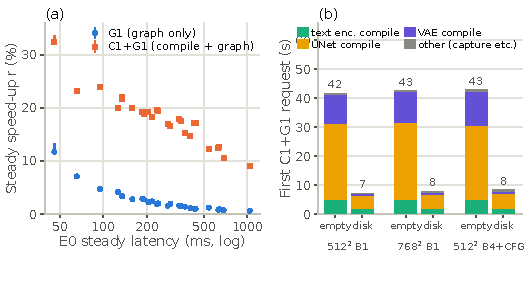
\includegraphics[width=0.5\linewidth]{../paper/figs/fig2_r_cost_v2.pdf}
\caption{(a)~Steady-state speed-up $r$ over eager of G1 (graph only) and C1+G1 versus eager latency (\NSTwoShapes{} shapes; bars: bootstrap CIs). (b)~First C1+G1 request at three shapes, stacked by component (first-call time of text-encoder, UNet and VAE compilation; \emph{other} = capture and residual first-call work) from an empty cache and from a warm disk cache; labels give seconds.}
\label{fig:cost}
\end{figure}
% AUTO-GENERATED by `python -m p24.paper.tab_metrics` -- do not edit by hand.  Every number is a \N... macro (numbers.tex).
\begin{table}[t]
\caption{Cost metrics per request shape on the main platform (SD1.5 + LCM-LoRA, fp16, four steps). B is the batch size, CFG the guided variant. Break-even counts are the numbers of requests that repay the one-time cost; brackets are confidence intervals (process bootstrap).}
\label{tab:metrics}
\centering\footnotesize
\setlength{\tabcolsep}{2pt}
\begin{tabular}{@{}lrrr@{}}
\toprule
Metric & 512$^2$, B1 & 768$^2$, B1 & 512$^2$, B4+CFG \\
\midrule
\multicolumn{4}{@{}l}{\emph{Steady-state latency (ms)}} \\
\quad E0 (eager) & \NTabISteadyEZeroFiveBOne & \NTabISteadyEZeroSevenBOne & \NTabISteadyEZeroFiveBFourCfg \\
\quad C1+G1 & \NTabISteadyCOneGOneFiveBOne & \NTabISteadyCOneGOneSevenBOne & \NTabISteadyCOneGOneFiveBFourCfg \\
\addlinespace[1pt]
\multicolumn{4}{@{}l}{\emph{Compile time (s)}} \\
\quad empty cache & \NTabICompileEmptyFiveBOne & \NTabICompileEmptySevenBOne & \NTabICompileEmptyFiveBFourCfg \\
\quad disk cache & \NTabICompileDiskFiveBOne & \NTabICompileDiskSevenBOne & \NTabICompileDiskFiveBFourCfg \\
\addlinespace[1pt]
\multicolumn{4}{@{}l}{\emph{First-request latency (s)}} \\
\quad E0 (eager) & \NTabIFirstEZeroFiveBOne & \NTabIFirstEZeroSevenBOne & \NTabIFirstEZeroFiveBFourCfg \\
\quad C1+G1, empty & \NTabIFirstCOneGOneEmptyFiveBOne & \NTabIFirstCOneGOneEmptySevenBOne & \NTabIFirstCOneGOneEmptyFiveBFourCfg \\
\quad C1+G1, disk & \NTabIFirstCOneGOneDiskFiveBOne & \NTabIFirstCOneGOneDiskSevenBOne & \NTabIFirstCOneGOneDiskFiveBFourCfg \\
\addlinespace[1pt]
\multicolumn{4}{@{}l}{\emph{Graph memory (MB)}} \\
\quad G1 pool & \NTabIPoolGOneFiveBOne & \NTabIPoolGOneSevenBOne & \NTabIPoolGOneFiveBFourCfg \\
\quad C1+G1 pool & \NTabIPoolCOneGOneFiveBOne & \NTabIPoolCOneGOneSevenBOne & \NTabIPoolCOneGOneFiveBFourCfg \\
\addlinespace[1pt]
\multicolumn{4}{@{}l}{\emph{Break-even count (requests)}} \\
\quad graph (G1) & \NTabIBreakGraphFiveBOne & \NTabIBreakGraphSevenBOne & \NTabIBreakGraphFiveBFourCfg \\
& {\scriptsize [\NTabIBreakGraphLoFiveBOne, \NTabIBreakGraphHiFiveBOne]} & {\scriptsize [\NTabIBreakGraphLoSevenBOne, \NTabIBreakGraphHiSevenBOne]} & {\scriptsize [\NTabIBreakGraphLoFiveBFourCfg, \NTabIBreakGraphHiFiveBFourCfg]} \\
\quad compile, disk & \NTabIBreakCompileDiskFiveBOne & \NTabIBreakCompileDiskSevenBOne & \NTabIBreakCompileDiskFiveBFourCfg \\
& {\scriptsize [\NTabIBreakCompileDiskLoFiveBOne, \NTabIBreakCompileDiskHiFiveBOne]} & {\scriptsize [\NTabIBreakCompileDiskLoSevenBOne, \NTabIBreakCompileDiskHiSevenBOne]} & {\scriptsize [\NTabIBreakCompileDiskLoFiveBFourCfg, \NTabIBreakCompileDiskHiFiveBFourCfg]} \\
\quad compile, empty & \NTabIBreakCompileEmptyFiveBOne & \NTabIBreakCompileEmptySevenBOne & \NTabIBreakCompileEmptyFiveBFourCfg \\
& {\scriptsize [\NTabIBreakCompileEmptyLoFiveBOne, \NTabIBreakCompileEmptyHiFiveBOne]} & {\scriptsize [\NTabIBreakCompileEmptyLoSevenBOne, \NTabIBreakCompileEmptyHiSevenBOne]} & {\scriptsize [\NTabIBreakCompileEmptyLoFiveBFourCfg, \NTabIBreakCompileEmptyHiFiveBFourCfg]} \\
\bottomrule
\end{tabular}
\end{table}


\subsection{Why Compilation Is Faster}\label{sec:mech-compile}



\begin{figure*}[t]
\centering
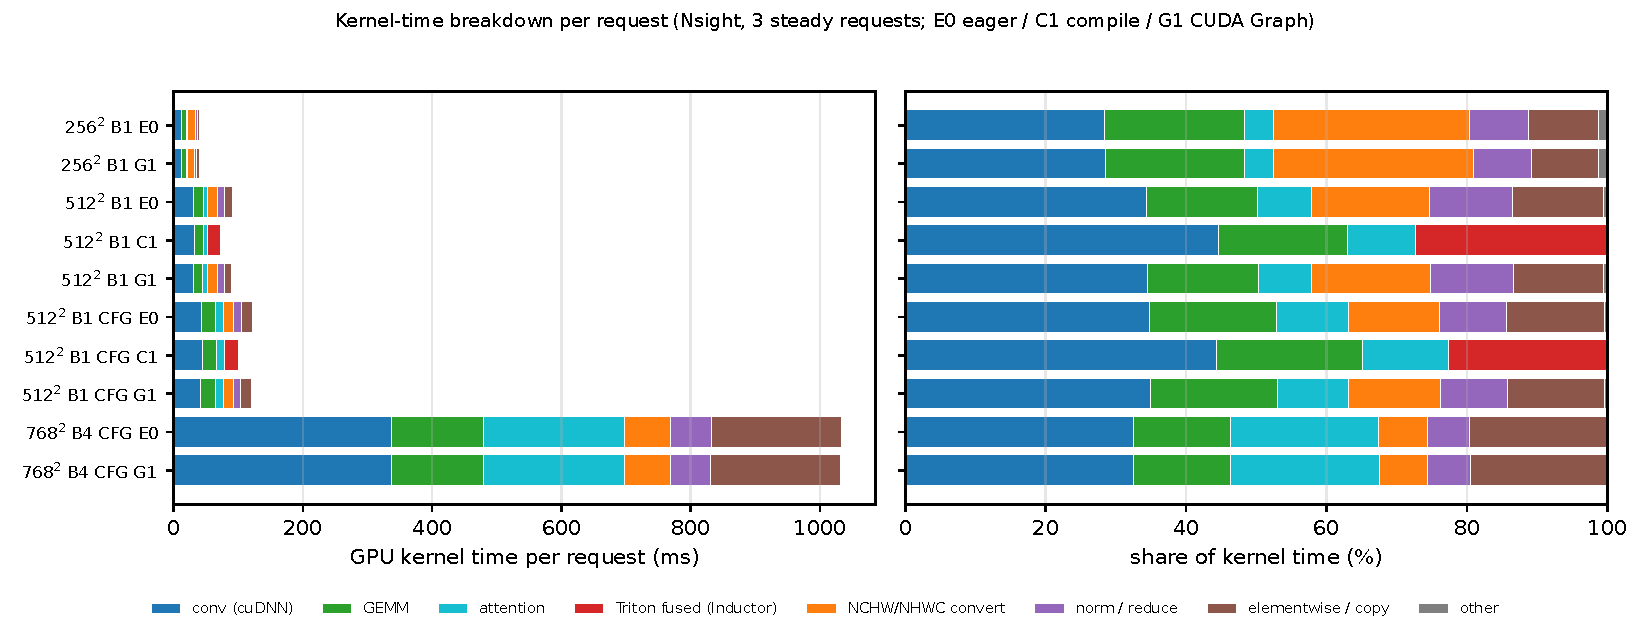
\includegraphics[width=0.6\linewidth]{../../results/S4X/ceiling/fig_kernel_breakdown.pdf}
\caption{GPU kernel time per request by kernel class for eager (E0), graph capture (G1) and compilation (C1) at three shapes (Nsight; C1 traces exist only at $512^2$). Compilation removes the layout-conversion, normalization and element-wise kernels and adds Triton-fused kernels; the large operators do not change. G1 has the same kernel composition as E0.}
\label{fig:kernels}
\end{figure*}

% src: internal:INT-01 (docs/internal_sources.md); results/S4X/ceiling/kernel_breakdown.csv
With CFG ($512^2$, batch one) the picture is the same: kernel time \tn{122.15} $\to$ \tn{101.23} ms (\tn{$-$17.1\%}), large operators \tn{+1.7\%}, \tn{15.84} ms of layout conversion gone.


% src: internal:INT-01 (docs/internal_sources.md)
\textbf{Ceiling.} If the large operators stay fixed and everything else vanished, compilation could save at most \tn{42.7\%} at $256^2$, \tn{40.6\%} at $512^2$ and \tn{32.4\%} at $768^2$ (batch four, CFG); measured steady-state savings are \tn{24.6\%}, \tn{20.3\%} and \tn{8.7\%}. The ceiling falls because the share of large operators in eager kernel time rises with size (\tn{52.5\%}, \tn{57.9\%}, \tn{67.5\%}). The ``large operators unchanged'' premise is verified only at $512^2$, the only shape with a C1 trace; at $256^2$ and $768^2$ it is an assumption.


% src: results/S4X/x10/verdict/verdict_X10.json; internal:INT-08 (docs/internal_sources.md)
\textbf{A second model.} To test whether these mechanisms are specific to one model, a pre-registered check (X10) repeated the cost and trace measurements on SD-Turbo (an SD2.1 distillation, one step, no CFG, fp16; same scripts, classes and idle-time definition; three processes per cell; judged at $512^2$ batch one). Lines fixed before the data: M1, compilation lowers total kernel time, large operators change by at most 3\%, and all other kernels account for at least 80\% of the net reduction; M2, the capture saving divided by derived idle time lies in [0.5, 1.5]. Both held. Compilation cut kernel time from \tn{48.3} to \tn{37.2} ms (\tn{22.9\%}); large operators changed by \tn{$-$0.6\%}; non-large kernels gave \tn{99\%} of the reduction (layout conversion alone an amount equal to \tn{62\%}). Capture saved \tn{2.20} ms against \tn{1.84} ms of derived idle time (ratio \tn{1.19}). The relative capture gain again fell with request time (\tn{8.3\%}, \tn{4.4\%}, \tn{0.9\%} at $384^2$, $512^2$ and $512^2$ batch four; reported only), and C1+G1 ran \tn{1.29}, \tn{1.35} and \tn{1.22}$\times$ faster than eager in steady state; all nine configuration cells passed equivalence. Serving results were not repeated on this model.

\section{Online Policy Details}\label{sec:online}
\begin{figure*}[t]
\centering
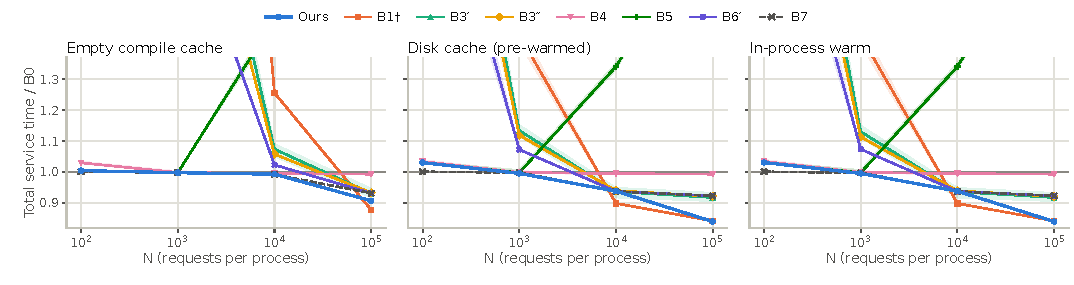
\includegraphics[width=0.68\linewidth]{../paper/figs/fig1_main.pdf}
\caption{Total service time relative to eager (B0) on W2 versus requests per process $N$, for three cold-start tiers (simulator; mean of ten evaluation seeds; baselines as in Sec.~\ref{m:method}, B6$'$ pre-builds the prior's most frequent shapes). $^\dagger$B1's simulated totals missed the pre-registered real-replay line (Sec.~\ref{sec:valid}).}
\label{fig:main}
\end{figure*}

\subsection{Primary Result: H4a Is Refuted}\label{sec:policy}
% src: internal:INT-02 (docs/internal_sources.md)
Fig.~\ref{fig:main} shows W2 total time relative to eager. B1 loses at small $N$ and from an empty cache but is the best online baseline at $N{=}10^4$ from the disk cache: B1 averages \NHfourABestSecTenK{} s and our policy \NHfourAOursSecTenK{} s, \NHfourAGapPctTenK\% slower (bootstrap 95\% CI [\NHfourABootLoPctTenK, \NHfourABootHiPctTenK]\%), by more than 2\% on \NHfourASeedsHigherTenK{} of \NHfourSeedsTotal{} seeds, so H4a is \NHfourAVerdictTenK. Relative to eager (Tab.~\ref{tab:policy}) the policy reaches \NTabWtwoOursTenK{} and B1 \NTabWtwoBOneTenK{}. H4b holds (W3: \NHfourBRatioTenK{} of B0) and H4c holds at $N{=}10^4$ (W1: \NHfourCRatioTenK{} of B1). At $N{=}10^3$, H4a is inconclusive (best online baseline B5, \tn{$-$0.20\%}) and H4c is refuted (\tn{1.0503}, 0/10 seeds within the line). Over the whole evaluation grid the policy is at most \tn{6.5\%} slower than B1 and at most \tn{9.3\%} slower than the best online baseline of each cell: a bounded worst case, not a speed-up.

% v1 HAND-TRIMMED COPY (2026-11-19) of the auto-generated tab2_policy.tex: tight-budget, simulator-validation and pending (TBD) blocks removed for the 4-page limit (their numbers are in the text); original file unchanged. Originally: AUTO-GENERATED by `python -m p24.paper.tab_policy`.  Every number is a \N... macro (numbers.tex);
% macros ending in TBD are placeholders for block C / recipe R (defined here, not registered).
\providecommand{\NTabCSimErrTBD}{\textbf{TBD}}
\providecommand{\NTabCSimVerdictTBD}{\textbf{TBD}}
\providecommand{\NTabRServeTBD}{\textbf{TBD}}
\providecommand{\NTabRServeCITBD}{\textbf{TBD}}
\begin{table}[t]
\caption{Policy versus baselines from the request-level simulator on the evaluation seeds, disk-cache tier. The dagger marks a baseline whose simulated totals were not confirmed by real replays. Ablation rows give the mean total service time in seconds.}
\label{tab:policy}
\centering\footnotesize
\setlength{\tabcolsep}{2.5pt}
\begin{tabular}{@{}lrrr@{}}
\toprule
\multicolumn{4}{@{}l}{\emph{Total time / B0, $N{=}10^4$}} \\
Workload & Ours & B1$^\dagger$ & B7 \\
\midrule
W1 & \NTabWoneOursTenK & \NTabWoneBOneTenK & \NTabWoneBSevenTenK \\
W2 & \NTabWtwoOursTenK & \NTabWtwoBOneTenK & \NTabWtwoBSevenTenK \\
W3 & \NTabWthreeOursTenK & \NTabWthreeBOneTenK & \NTabWthreeBSevenTenK \\
\midrule
\multicolumn{4}{@{}l}{\emph{Hypotheses (primary cell)}} \\
H4a (W2), vs.\ best online & $+$\NHfourAGapPctTenK\% & [\NHfourABootLoPctTenK, \NHfourABootHiPctTenK] & \NHfourAVerdictTenK \\
H4b (W3), Ours / B0 & \NHfourBRatioTenK & & \NHfourBVerdictTenK \\
H4c (W1), Ours / B1 & \NHfourCRatioTenK & & \NHfourCVerdictTenK \\
\midrule
\multicolumn{4}{@{}l}{\emph{Ablation (mean total time, s)}} \\
Variant & W2 & W5 & \\
\quad Ours (full) & \NTabAblOursWtwoSec & \NTabAblOursWfiveSec & \\
\quad three tiers & \NTabAblThreeTiersWtwoSec & \NTabAblThreeTiersWfiveSec & \\
\quad LRU eviction (B5) & \NTabAblLruWtwoSec & \NTabAblLruWfiveSec & \\
\quad no prior & \NTabAblNoPriorWtwoSec & \NTabAblNoPriorWfiveSec & \\
\quad B0 (eager) & \NTabAblBZeroWtwoSec & \NTabAblBZeroWfiveSec & \\
\bottomrule
\end{tabular}
\end{table}



\subsection{How Much Could Any Online Selection Save?}\label{sec:ceiling}
% src: internal:INT-01 (docs/internal_sources.md)
The refutation could mean that our policy is poorly tuned, or that there is little to win. We separate the two by post-hoc accounting (computed after H4a was judged; it does not change any verdict). First, a hard ceiling: a policy that never does worse than eager on a shape and keeps all of B1's steady-state gain can save at most B1's one-time cost. We rebuilt B1's total from the cost table and the traces; it matches the simulator to \tn{0.000 s} on every seed. Second, a tighter estimate: an oracle that knows every shape's count in advance and chooses compile or eager per shape (no memory limit, no capture; coordinate descent, a local optimum). Tab.~\ref{m:tab:ceiling} gives the result: on W2 the hard ceiling is \tn{43.9\%} of B1's time at $N{=}10^3$ (where eager is the oracle's choice) and \tn{7.34\%} at $10^4$, where the oracle saves only \tn{0.83\%} (it leaves \tn{9.2} rare shapes eager). Compiled components are shared across shapes, so the oracle is not guaranteed to be global.




\subsection{Further Online Attempts}\label{sec:attempts}
% src: internal:INT-06 (docs/internal_sources.md); internal:INT-07 (docs/internal_sources.md)
The revised admission rule v3 (``affordable zone'' with posterior admission) is summarized in Sec.~\ref{m:online} and row 15 of App.~\ref{app:attempts}; its design was revised once after development numbers (App.~\ref{app:dev}). The other attempts:




% src: internal:INT-07 (docs/internal_sources.md); internal:INT-06 (docs/internal_sources.md)
\textbf{Hiding the compile in the background.} If one-time cost cannot be avoided, perhaps it can be hidden. In simulation, background compilation with eager service meanwhile would reach \tn{0.9419} of B1 on W2 at $N{=}10^4$ (assuming eager slows by at most $f{=}0.1$). On the GPU, during the roughly 6 s compile window eager requests were slowed by $f{=}$\tn{8.6} extra (about \tn{9.6}$\times$ normal time; \tn{8.47}/\tn{8.49}/\tn{8.92}; line $\le$0.3), single requests reaching \tn{3.4--3.6 s}. Re-simulating with the measured $f$ gives \tn{0.9983}, i.e.\ no gain. The evidence points to GIL contention (convoy effect) between the compile thread and the serving thread: shortening the interpreter switch interval from 5 to 0.05 ms only reduced $f$ to \tn{3.5}. Serving the shape from a graph while it compiles fails in simulation (the graph budget holds about five graphs, so most traffic still runs eagerly and slowed); even with a zero-interference graph path the line is missed while eager suffers $f{=}8.6$. A pre-warm in a subprocess gave no gain from the disk tier (\tn{1.0066}), because the main process still blocks for about \tn{5.8 s} loading the result.

% src: internal:INT-07 (docs/internal_sources.md); internal:INT-06 (docs/internal_sources.md)
\textbf{A faster steady state through tuning.} The official Inductor diffusion recipe (coordinate-descent tuning) is faster in steady state but paid \tn{37--60 s} more than plain compilation on each new process's first request per shape. The cause is a known upstream issue, a lost \texttt{found\_by\_coordesc} flag~\cite{pt_issue,pt_pr}, which in our runs made coordinate descent re-run on \tn{102} of \tn{203} kernels in every new process; we located it independently but do not claim to have found it. A configuration-only workaround (two public environment variables and one settling compile per shape) cut the warm first request to \tn{6.5--15.3 s} while keeping a \tn{3--5\%} steady-state gain with 6/6 equivalence. On real replays B1 with the recipe still took \tn{1.088}$\times$ the total time of plain B1 (CI [\tn{1.069}, \tn{1.114}]): each new shape's first request costs about \tn{0.6 s} more, which outweighs a \tn{4--5\%} steady-state gain at $N{=}300$. ``Faster in steady state'' is not ``faster as a service''.


\subsection{Admission, Eviction, Padding and Memory Mechanisms}
% src: internal:INT-02 (docs/internal_sources.md); internal:INT-03 (docs/internal_sources.md)
Both memory mechanisms did almost nothing on the 4090: padding was never triggered, since no measured shape was both equivalent and faster; graph eviction changed total time by at most \tn{0.05\%}, since the graph layer is worth little; plain LRU (B5) thrashes and ends slower than eager (\NTabAblLruWtwoSec{} s against \NTabAblBZeroWtwoSec{} s). Under a tight \NTabTightBudgetGB{} GB budget the policy still trails B1, which has no graph pool. Dropping the prior or a tier changes W2 time by a few percent (Tab.~\ref{tab:policy}). The cost model predicts, and the H200 confirmed (Sec.~\ref{sec:h200}), that padding does pay on a platform with faster eager and slower compilation (\tn{8 of 9} combinations): the uselessness of these mechanisms is a property of this platform and model, not of the mechanisms.

% src: internal:INT-09 (docs/internal_sources.md); results/S5/rare_evict/x5_evictions.csv; internal:INT-02 (docs/internal_sources.md); results/S5/rare_evict/rare_shape_summary.csv
\textbf{Eviction and rare shapes on real hardware} (summary in Sec.~\ref{m:online}). In the $N{=}10^4$ replay (X5) each policy process evicted its \tn{6} graphs between requests \tn{2632} and \tn{4254}, each freeing within \tn{4--18} MB of its accounted size; four further releases per process were tier upgrades (a graph replaced by a compile+graph one), not evictions. The allocator's reserved peak (\tn{20540} MB) exceeded the simulator's estimate by \tn{786} MB, the whole-process effect of App.~\ref{sec:mem}. From an empty cache (X8) B1's rare-shape first requests reached \tn{42.5 s} at most and cost \tn{+232 s} over eager per stream; the policy matched eager within \tn{0.03 s}. With packages on disk the full AOT set paid about \tn{1 s} per rare shape to load its package (\tn{+1.0--2.9 s} per stream over eager), whereas the bounded set, which leaves rare shapes eager, matched eager (\tn{+0.0--0.1 s}). A 0.5\% rarity threshold gives the same ordering.

\subsection{Regime Map Relative to B1 and the $N{=}10^4$ and Empty-Cache Replays}\label{sec:regime}
% src: internal:INT-10 (docs/internal_sources.md); results/S4X/x5/verdict/e12_verdict.json; results/S4X/x9/verdict/h123_verdict.json; results/S4X/x8/verdict/h12_verdict.json; internal:INT-16 (docs/internal_sources.md)
We swept $N\in\{10^2,300,10^3,3\cdot10^3,10^4\}$, both cache tiers, four workloads and two budgets with the frozen simulator (descriptive; reuses the H4 evaluation seeds). From the disk tier B1 breaks even with eager at $N{\approx}$\tn{4.3k} on W2/W5 (\tn{3.5k} with the calibrated cost model) and \tn{380} (\tn{290}) on the one-shape W1, and is \tn{1.9--2.6}$\times$ slower than eager at $N{=}300$. Our policy beats B1 below $N{\approx}3000$ and loses above it (crossing \tn{3.2--4.4k} on W2/W5, \tn{2.1--2.2k} on W3); against eager it is \tn{0.994--1.033} for $N{\le}10^3$, \tn{1--6.4\%} slower at $N{=}3000$ and about \tn{6--7\%} faster at $10^4$, where B1 (\tn{0.89--0.90}) is faster still. Of 34 real-replay ratios at $N{\le}10^3$, \tn{33} lie on the predicted side of 1 (the exception is a tie, \tn{1.0009} vs.\ \tn{0.9995}); the seven later pre-registered ratios all do (\tn{40 of 41}). X5 (W2, seed 133, three processes per policy): B1 \tn{1931 s}, policy \tn{2017 s} (\tn{4.5\%} slower; paired ratios \tn{1.038--1.054}; predicted \tn{4.3\%}; errors \tn{1.6\%} and \tn{1.8\%}); one process ran while host load rose to about 27, and excluding it gives \tn{1.040--1.043}. X9 added eager (\tn{2140.8 s}) and AOT (\tn{0.845} of eager, all three pairs) on the same stream a day later; one bridge process per policy differed from X5 by \tn{$-$0.2\%} (B1) and \tn{$-$0.7\%} (policy), within the pre-set 2\%. From an empty cache (simulated, mostly interpolated) the policy is \tn{21\%} (W2/W5) and \tn{10\%} (W3) faster than B1 at $N{=}10^4$ (\tn{6--17\%} under four calibrations, App.~\ref{app:calib}). X8 (W2, $N{=}10^3$, seed 135, a new empty cache per process): B0 \tn{213.2 s}, policy \tn{212.5 s}, B1 \tn{947.2 s}; B1 compiled all \tn{31} shapes and its first request took \tn{38.1--38.7 s}, whereas the policy kept \tn{30} shapes eager, captured one graph and answered its first request in \tn{0.65--0.70 s}.

\section{Offline Route Details}\label{sec:offline}
\subsection{AOT Packages at $N{=}300$: Half the Answer}\label{sec:fail}
% src: internal:INT-10 (docs/internal_sources.md); internal:INT-06 (docs/internal_sources.md); internal:INT-05 (docs/internal_sources.md); internal:INT-07 (docs/internal_sources.md)
If one-time cost is the bottleneck, move it offline. We built AOTInductor~\cite{pt_aoti} packages for the 32 prior shapes (about \tn{35 min}, eight threads, not counted in service time; B0 needs no offline work) and replayed fresh real streams from the disk tier (packages on disk). Three lines were fixed beforehand: A1, B1-AOT/B1; A2, first-request median; A3, B1-AOT/B0 $\le$0.90. At $N{=}300$, total time falls to \tn{0.423} of B1 (A1 holds) and the first request of a new shape takes a median \tn{0.59--0.61 s} (A2 holds), but against eager AOT only ties, \tn{0.985} (A3 \emph{not} met). The mechanism is visible in the split: AOT's remaining one-time cost (\tn{19--22 s} per process, against \tn{119--128 s} for B1, steady state identical) is about as large as its steady-state saving over eager at 300 requests. From an empty cache AOT is more expensive than plain compilation (\tn{62--69 s} to build a package per shape against \tn{25--45 s} for a cold compile). By the pre-registered rule, no real end-to-end speed-up was claimed at this point.


\subsection{A Bounded Set of Buckets}
% src: internal:INT-03 (docs/internal_sources.md); internal:INT-02 (docs/internal_sources.md)
Do fewer packages suffice? The brief asks for a bounded set of buckets with eager fallback. A rule fixed before evaluation ranks shapes by expected net saving at $N{=}10^3$ (prior half of DiffusionDB, cost table) and stops at 50\% of the full build time: $K{=}15$ of 32 shapes, \tn{985 s} of \tn{2096 s}, covering \tn{84\%} of prior requests; the rest run eagerly. On a fresh real stream (seed 131; W2, W5; $N{=}10^3$; three processes per arm) the set serves in \tn{0.9943}/\tn{1.0024} of the full set's time (K1, line $\le$1.02, met) with \tn{16--18\%} of requests eager. With the offline build counted as in a cold start, total time is \tn{0.5144}/\tn{0.5156} of the full set's (K3, line $\le$0.5642, met), though \tn{5.4}$\times$ eager's. Against eager the set needs \tn{0.892}/\tn{0.896} of the time (K2; reported, not judged). The simulator was within \tn{0.81\%} (K4), and on ten further simulated seeds (140--149) both lines held for both streams (10/10). At $N{=}10^4$ (simulated, not judged) the set is \tn{3.6\%} slower than the full set, so building everything wins there.



\subsection{When Does Building Ahead Pay? Amortization and Regime}
% src: internal:INT-10 (docs/internal_sources.md)
Fig.~\ref{m:fig:regime} gives the conditions. From the disk tier B1-AOT breaks even with eager at $N{\approx}$\tn{245--306} (W2, W3, W5), is \tn{13--26\%} slower at $N{=}100$, \tn{10.6--11.2\%} faster at $10^3$ and \tn{13.4--15.7\%} faster at $10^4$ (simulated); the bounded set breaks even at $N{\approx}$\tn{120--180} and is the best arm at $N{=}300$ on W2/W5. If instead every process builds its own packages, AOT never pays: at $N{=}10^4$ the bounded set needs \tn{1.2--1.8}$\times$ and the full set \tn{1.5--3.0}$\times$ eager's time. The build pays off once it is shared: against eager, the full set needs about \tn{6.3} processes at $N{=}10^4$ and \tn{87} at $10^3$; the bounded set \tn{3.7} and \tn{41}; at $N{=}300$ over 600. Building ahead is thus a deployment decision (``build once, reuse in many processes''), and the bounded set mainly cuts the number of processes needed to amortize it.

% src: internal:INT-01 (docs/internal_sources.md)
\textbf{Ceiling after AOT.} Assuming about \tn{0.5 s} of online one-time cost per shape once packages exist (an assumption, not a measured split), the 32 shapes cost about \tn{16 s} per process; at $N{=}10^4$ any online selection could then save at most about \tn{0.9\%} relative to B1-AOT. AOT removes almost all of the one-time cost that online selection was trying to manage.

% src: internal:INT-03 (docs/internal_sources.md)
\textbf{Tuned kernels in the packages.} A conditional attempt, building the recipe's tuned kernels into the packages, was pre-registered to run only if the margin of the $N{=}10^3$ result to its line were below 1\%; the margin was \tn{1.10\%}, so it was not triggered.

% src: internal:INT-03 (docs/internal_sources.md); internal:INT-17 (docs/internal_sources.md); internal:INT-02 (docs/internal_sources.md)
\textbf{Second platform.} The offline route was also tested, pre-registered, on an H200 (never mixed with 4090 numbers). On the node we measured a reduced cost table (eager, compile and AOT for 31 shapes), let the frozen predictor forecast each policy's total time before any replay, and replayed the W2 stream (seed 130) with three processes per arm. At $N{=}10^3$ the AOT packages needed \tn{0.760} of eager's total time (H1, line 0.90: met; \tn{0.895} at $N{=}300$, reported only), and the predictions were within \tn{1.5\%} (eager) and \tn{1.9\%} (AOT) of the measured totals (H2, line 5\%: met; all six cells within \tn{3.8\%}). Building ahead therefore also pays on a platform where eager is faster and compilation repays later, with the same proviso as on the 4090: the 30 packages took \tn{59 min} to build (one of the 31 shapes, $512^2$ at batch three without CFG, had no package and ran eagerly, \tn{4.1\%} of requests, above the pre-set 3\% validity flag; the verdict is unchanged), and with that build charged to a single process the total is \tn{20.4}$\times$ eager's.


\section{Memory Details}\label{sec:mem}
% src: internal:INT-07 (docs/internal_sources.md); internal:INT-02 (docs/internal_sources.md); internal:INT-06 (docs/internal_sources.md)
\textbf{The graph pool is bounded, the process is not.} The policy keeps its graph pools within budget (\tn{5686} MB against \tn{6565} MB), yet whole-process peak memory reached \tn{20140} MB, and B1, which has no graph pool, measured \tn{8.8--10.7 GB} against \tn{7.1 GB} predicted. The cause is the caching allocator: reserved memory accumulates as shapes are compiled (B1 on W2: \tn{5388} MB at request 30, \tn{10958} MB after compiling the largest shape) while allocated memory stays near \tn{2.02 GB}. Graph-pool accounting is correct; the process simply holds more. (Generic memory advice for diffusion pipelines~\cite{hf_memory} addresses model memory, not this accumulation.)

% src: results/S4/mem_43b/fit/verdict.json (n_cells_pass 4 / 13); internal:INT-06 (docs/internal_sources.md)
\textbf{Attempt 1: a better memory model.} A refit predicting whole-process peaks from per-shape accumulation terms had to be conservative and within 1 GB in all 13 cells; it met this in \tn{4} of 13 (out of sample \tn{2} of 11). Verdict: not repaired; whole-process peaks are reported only as measured upper bounds.

% src: internal:INT-03 (docs/internal_sources.md)
\textbf{Attempt 2: a mechanism instead of a model.} A pre-registered cap bounded the whole process: an allocator limit $C{=}16384$ MiB (\texttt{torch.cuda.set\_per\_process\_memory\_fraction}, which limits only PyTorch's caching allocator~\cite{pt_memfrac}; the CUDA context and library workspaces lie outside it, so we judge whole-process peaks by NVML with a margin $\delta$) with a garbage-collection threshold of 0.8, the graph-pool budget fitted inside $C$, and the device-level line $C{+}\delta$ (\tn{18102} MB; $\delta{=}$\tn{1718} MB, the memory the allocator does not see, frozen from development runs). Four lines: M1 peak $\le C{+}\delta$; M2 no crash; M3 outputs bit-identical with and without the cap; M4 time ratio $\le$1.03. On fresh streams (seed 132; W2, W5; $N{=}300$; our policy and the capture-on-first-sight baseline B4; three processes per version) capped peaks were \tn{15.7--16.2 GiB} against \tn{19.9--21.9 GiB} uncapped, with no crash and time ratios \tn{0.9975--1.0024}. Outputs were bit-identical for our policy on both streams and for B4 on W2, but for B4 on W5 one request per process (request 30, the largest shape, $768^2$ batch four with CFG, served eagerly) changed, identically in all three processes. That cell failed M3, so the pre-registered verdict is \textbf{FAILS} (three of four cells pass).

% src: internal:INT-13 (docs/internal_sources.md); internal:INT-03 (docs/internal_sources.md)
\textbf{Why the output changed.} An exploratory probe (not a verdict) replayed that stream with an allocator out-of-memory observer. Under the cap, request 30 triggers \tn{29} allocator failures, each a \tn{2306} MiB request from \texttt{Conv2d.forward} (the cuDNN convolution workspace) while device usage sits at the cap; the framework catches the failure and falls back to another convolution algorithm, which changes the numerics slightly. Without the cap there are no failures. Fixing the cuBLAS workspace, capping the cuDNN workspace through an environment variable (not recognized by our cuDNN~9.10), or disabling benchmarking with deterministic algorithms did not help. Switching the allocator to expandable segments (\texttt{expandable\_segments} in \texttt{PYTORCH\_CUDA\_ALLOC\_CONF}, documented by PyTorch as experimental~\cite{pt_alloc_conf}) did: with the cap and the same garbage-collection threshold, all 300 requests were bit-identical to the uncapped run, with no allocator failure, and the allocator's peak reserved memory fell from \tn{21204} to \tn{12434} MB; uncapped outputs were unchanged by the setting. Because this changes the allocator recipe, the memory numbers had to be re-measured under a new card frozen before its confirmation data (X2b: expandable segments, same 16~GiB cap, $\delta{=}$\tn{1882} MB, seed 134), all four cells (W2, W5 $\times$ our policy, B4) passed: whole-process peaks (NVML) fell from \tn{19.7--20.7} GiB uncapped (default allocator) to \tn{13.1--13.3} GiB, there were no crashes and no allocator failures, all \tn{900} compared requests per cell (three process pairs $\times$ 300) were bit-identical to the uncapped run, and time ratios were \tn{0.997--0.999}. The cap was never reached (the same recipe without a cap peaked at the same level), so it acts only as insurance. On the same stream the original X2 recipe again triggered \tn{29} allocator failures and \tn{5} changed images in W2/B4, which the new recipe removed. The caveat remains: when a cap does bind a convolution workspace, cuDNN switches algorithm and outputs change; X2 stays FAILS as recorded, and a check at $C{=}10240$ MiB reproduced the switch (\tn{56} allocator failures, \tn{2--3} of 300 images changed).

\textbf{What we claim.} The cache is graph-pool-bounded and process-capped, with a known numerical caveat; the cap costs no measurable time. Bit-identity under a binding cap is not guaranteed by PyTorch's default allocator on this stack, and we report that as a finding rather than hide it.


\section{Validation, Quality and Second Platform}\label{sec:trust}
\subsection{Simulator Validation and Error Analysis}\label{sec:valid}
% src: internal:INT-02 (docs/internal_sources.md); internal:INT-07 (docs/internal_sources.md); internal:INT-05 (docs/internal_sources.md); internal:INT-03 (docs/internal_sources.md); results/S4X/x5/verdict/e12_verdict.json; results/S4X/x8/verdict/h12_verdict.json
The pre-registered validation replayed three streams (W2, W3, W5; $N{=}300$; three processes per policy) against a 10\% total-time line. Orderings were reproduced (\tn{all 13 non-tied}) and steady-state costs matched within \tn{1.5\%}, but the line failed: B1 reached \NRealMaxErrPct\% (W2) and \NRealErrBOneWthreePct\% (W3), the policy \NRealErrOursWtwoPct\% and \NRealErrOursWthreePct\%. All \NRealJudged{} cells were over-predicted. Two causes: unmeasured in-process one-time costs fell back to cold-start bounds (about one third of B1's error), and compilation ran about \tn{13--17\%} faster than in the cost table, of which host load explains at most about \tn{8\%} (Spearman $\rho{=}$\tn{0.44}; the remainder is unexplained). This over-prediction penalizes compilation, so it makes the refutation of H4a more secure, not less. Simulator v2 (measured in-process costs, structural corrections), frozen before the data, was then tested on fresh replays (seed 101, $N{=}300$): \tn{all 16 cells within 10\%, maximum 2.26\%, 17 of 17 non-tied orderings}. Later predictions were within \tn{0.48\%} (AOT, $N{=}10^3$) and \tn{0.81\%} (bounded set). At $N{=}10^4$ (X5, real replay) the errors were \tn{1.6\%} (B1, predicted \tn{1899 s}, measured \tn{1931 s}) and \tn{1.8\%} (policy, \tn{1982 s} vs.\ \tn{2017 s}); both under-predicted by about \tn{2\%}, the first validation point beyond $N{=}10^3$. From an empty cache (X8, $N{=}10^3$; the frozen cost model, with missing empty-tier costs interpolated) the simulator over-predicted every policy: by \tn{4.3\%} for B0 and our policy and by \tn{13.0\%} for B1 (\tn{1070 s} predicted, \tn{947 s} measured), all under the 15\% marker of that card; B1's larger error matches the \tn{13--17\%} faster compilation found above.

\subsection{Image Quality}\label{sec:quality}
% src: internal:INT-03 (docs/internal_sources.md); results/S4X/x4/analysis/geneval_S4X_X4_verdict.txt
GenEval~\cite{geneval} (553 prompts, four images each, $512{\times}512$) checks that quality is unchanged against a pre-registered $\pm0.02$ band. Eager scores \NGenEvalEZeroOverall{} Overall (95\% CI [\NGenEvalEZeroCiLo{}, \NGenEvalEZeroCiHi{}]); C1+G1 differs by \NGenEvalCOneGOneDelta{} ([\NGenEvalCOneGOneCiLo{}, \NGenEvalCOneGOneCiHi{}]), the padding variant by \NGenEvalPadDelta{} ([$-$0.0056, +0.0026]) and the AOT packages by \tn{$-$0.0006} ([$-$0.0044, +0.0032]), all inside the band. With CFG (guidance 1.5) eager scores \tn{0.355} and C1+G1 differs by \tn{+0.0006} ([$-$0.0037, +0.0052]), also inside. For reference, the GenEval paper reports 0.43 Overall for SD1.5 at its default settings (Table~2 of~\cite{geneval}); our eager reference is a 4-step LCM-LoRA sampler at guidance 1.0, so the settings differ and the two numbers are not compared directly, and our claim concerns only paired differences to eager. Other resolutions and batch sizes have numerical equivalence only, not a task-level quality check.

\subsection{Second Platform (H200)}\label{sec:h200}
% src: internal:INT-06 (docs/internal_sources.md); internal:INT-03 (docs/internal_sources.md)
An H200 was used only to test whether the cost model transfers; its numbers are never mixed with the 4090's (Tab.~\ref{tab:h200}). Equivalence passed 8/8. C1+G1 was \tn{2.75}$\times$ (512$^2$, batch one) and \tn{1.53}$\times$ (batch four, CFG) faster than eager in steady state, against \tn{1.32}$\times$/\tn{1.17}$\times$ on the 4090; because eager is faster and compilation slower, C1+G1 repays later (disk tier \tn{357}/\tn{331} requests against \tn{301}/\tn{131}). A pre-registered job on \tn{14} unseen cells confirmed three predictions of the cost model: padding pays on the H200 (\tn{8 of 9} combinations; never on the 4090), two named cells have CIs excluding zero, and compilation repays later than on the 4090 (\tn{14 of 14}). In the first run \tn{5 of 24} empty-cache processes (40 in all) failed while reading Triton cache files from the cluster's network file system during empty-cache compiles; a rerun on node-local disk had \tn{0 of 24} failures, supporting a file-system race, but its first requests were \tn{19--25\%} faster than in the reference, outside the $\pm$10\% line, so that check FAILS as recorded.

\begin{table}[t]
\caption{Second-platform test of the cost model (H200; never pooled with 4090 numbers). Break-even: C1+G1, disk tier, $512^2$ batch one / batch four with CFG.}
\label{tab:h200}
\centering\footnotesize
\setlength{\tabcolsep}{3pt}
\begin{tabularx}{\columnwidth}{@{}Yll@{}}
\toprule
Quantity & 4090 & H200\\
\midrule
% src: internal:INT-06 (docs/internal_sources.md)
C1+G1 steady speed-up over E0 & \tn{1.32}$\times$ / \tn{1.17}$\times$ & \tn{2.75}$\times$ / \tn{1.53}$\times$\\
% src: internal:INT-06 (docs/internal_sources.md)
Break-even requests (C1+G1) & \tn{301} / \tn{131} & \tn{357} / \tn{331}\\
% src: internal:INT-03 (docs/internal_sources.md)
Padding pays (predicted on H200) & never & \tn{8/9} (PASS)\\
% src: internal:INT-03 (docs/internal_sources.md)
Repays later on H200 (predicted) & -- & \tn{14/14} (PASS)\\
% src: internal:INT-03 (docs/internal_sources.md)
Node-local empty-cache rerun: failures & -- & \tn{0/24}\\
% src: internal:INT-03 (docs/internal_sources.md)
\quad first request vs.\ reference & -- & \tn{19--25\%} faster (FAIL)\\
% src: results/S4P/p5d/verdict/d123_verdict.json; internal:INT-03 (docs/internal_sources.md)
AOT/B0, $N{=}10^3$ (H1/H2) & \tn{0.890} & \tn{0.760} (PASS/PASS)\\
\bottomrule
\end{tabularx}
\end{table}


\section{Failure Catalogue and Graph-Invalidation Analysis}\label{sec:failures}
% src: internal:INT-02 (docs/internal_sources.md); internal:INT-06 (docs/internal_sources.md)
The brief asks for an analysis of graph-invalidation failures. Tab.~\ref{tab:failures} lists what invalidated or broke a compiled or captured artifact in this project, with its trigger, consequence and countermeasure; each row has a regression test or a result file in the repository. Three groups emerge. \emph{Shape and value changes} (rows 1--5) are the expected invalidations: every new key (height, width, batch, CFG, step count) needs a new compile and a new graph, and two silent paths exist---a Python-float guidance value recompiles per value, and beyond the default recompile limit new shapes silently run eagerly. \emph{Hidden state} (rows 6--8) breaks capture without an error message: host-side scheduler state, captured addresses, and the tensor kind (inference vs.\ normal) as part of the guard. \emph{Resource conditions} (rows 9--14) are the costly ones in a service: graph pools that accumulate until the device is full, capture under memory pressure, host pinned-memory failures, network-file-system cache races, and allocator failures that change cuDNN's algorithm. Eviction has a price as well: re-capturing an evicted graph took \tn{5.6--13.1}$\times$ the bare capture time in wall-clock terms (reserved memory returned to within \tn{44 MB} of its pre-capture level), which the eviction rule charges as rebuild cost.

\begin{table*}[t]
\caption{Graph-invalidation and failure catalogue (selected rows of the full catalogue in the repository; 4090 unless marked).}
\label{tab:failures}
\centering\scriptsize
\begin{tabularx}{\textwidth}{@{}rP{3.2cm}YY@{}}
\toprule
\# & Trigger & Consequence & Countermeasure\\
\midrule
1 & Shape change & \texttt{dynamic=False}: one compile per distinct shape; a manual graph cannot take another shape (copy size mismatch; replay keeps the captured shape) & One key (H, W, B, CFG) $\to$ one compile and one graph set\\
2 & Guidance as Python float & One graph per distinct value under static shapes & Keep guidance as a 0-dim tensor\\
3 & Step count / scheduler change & One graph per distinct count; a 4-step graph always replays 4 steps & Step count is part of the key (fixed 4-step loop)\\
4 & Recompile limit (default 8) & With \texttt{fullgraph=False} the 9th and later shapes silently run eager; with \texttt{fullgraph=True} an exception & \texttt{recompile\_limit=64} for B1; default kept as baseline B3$'$\\
% src: internal:INT-04 (docs/internal_sources.md)
5 & Padding to a shared bucket & 1 of 6 padded cells not equivalent ($512^2$, batch 3$\to$4, RMSE ratio \tn{2.665}) & Padding only where equivalent and faster (never on the 4090)\\
6 & Scheduler state on the host & Python step index, CPU tables and in-step RNG are not captured & Re-implemented 4-step loop with device-resident constants, noise drawn before the request (bit-exact vs.\ diffusers)\\
7 & Captured inputs need stable addresses; graph-tree outputs reused & New tensors are not read by replay; outputs overwritten by the next replay & Static buffers with \texttt{copy\_} in, \texttt{clone()} out; step-begin marker per request\\
% src: internal:INT-04 (docs/internal_sources.md)
8 & Tensor kind in the guard & Inputs created outside \texttt{inference\_mode} compiled the UNet twice per shape; upgrading C1$\to$C1+G1 recompiled once (\tn{+3.8 s}) & Create inputs under \texttt{inference\_mode}; swap buffers for inference clones\\
% src: internal:INT-04 (docs/internal_sources.md)
9 & Graph pools accumulate & G1 without release: OOM at the 10th of 12 shapes with \tn{19.24 GiB} in private pools & Budgeted capture; eager when over budget; evict and retry\\
10 & Capture under memory pressure / no per-shape release API & Capture raises OOM; \texttt{torch.compiler.reset()} frees all shapes & Manual per-shape pools with release; budget = cap $-$ resident $-$ eager peak $-$ margin\\
% src: internal:INT-04 (docs/internal_sources.md)
11 & Large-shape cold compile ($768^2$, batch four, CFG) & Failed with \texttt{cudaErrorInvalidValue} in 5 of 10 empty-cache processes (plus 2 pre-warm attempts) before a host reboot; 0 of 3 after & Inductor backs up a \tn{1152 MiB} buffer in pinned host memory, refused in a degraded host state; compile large shapes offline; pageable fallback\\
% src: internal:INT-07 (docs/internal_sources.md)
12 & Lost tuning flag (official recipe) & Coordinate descent re-runs on \tn{102/203} kernels per new process (+\tn{37--60 s}) & Known upstream issue~\cite{pt_issue}; configuration workaround\\
% src: internal:INT-03 (docs/internal_sources.md)
13 & H200 network file system & \tn{5 of 24} empty-cache processes (40 in all) failed reading Triton cache files during compilation & Node-local disk: \tn{0 of 24}\\
% src: internal:INT-03 (docs/internal_sources.md); internal:INT-13 (docs/internal_sources.md)
14 & Allocator cap binds a cuDNN workspace & \tn{29} failed \tn{2306 MiB} requests; cuDNN falls back to another algorithm; output changes & Expandable segments; confirmed under a new card (X2b, 4/4 cells bit-identical, peaks \tn{13.1--13.3 GiB})\\
% src: internal:INT-08 (docs/internal_sources.md)
15 & AOT packages combined with graph capture & Capture failed at CFG shapes: with the default capture mode both probed shapes failed with \texttt{operation not permitted when stream is capturing}; with a relaxed capture mode the $512^2$ no-CFG shape captured, but the $768^2$ CFG shape still failed with \texttt{operation not permitted on an event last recorded in a capturing stream} (an exploratory AOT side run). Cause, from the AOTInductor runtime: each package call queries the event its previous call recorded, and with CFG the text encoder is called twice in one capture & AOT arms (and their GenEval check) run without capture. A later probe captured only the UNet package, once per capture, or loaded it single-threaded: all three probed shapes captured with bit-identical images but gained only \tn{0.2--2.2\%} in steady state (App.~\ref{app:attempts}, row 36)\\
16 & Driver exception class & Frozen driver catches an exception class the runtime lacks: a real capture OOM would raise \texttt{AttributeError} instead of falling back & Capture failures were zero in the $N{=}300$ and $N{=}10^3$ real replays, so those data are unaffected\\
\bottomrule
\end{tabularx}
\end{table*}

\section{All Attempts}\label{app:attempts}
Every attempt to speed up the service or to repair a failed check, in project order. ``Line'' is the decision line fixed before the deciding data; ``Result'' gives the verdict as recorded. Sim = simulator; real = real replay on the 4090.

{\scriptsize
\setlength{\tabcolsep}{2pt}
\begin{longtable}{@{}P{0.4cm}P{2.2cm}P{2.6cm}P{2.6cm}P{3.3cm}P{3.2cm}P{2.2cm}@{}}
\toprule
\# & Attempt & Hypothesis & Line & Result (verdict) & Mechanism / evidence & Next\\
\midrule
\endfirsthead
\toprule
\# & Attempt & Hypothesis & Line & Result (verdict) & Mechanism / evidence & Next\\
\midrule
\endhead
\bottomrule
\endfoot
% src: internal:INT-01 (docs/internal_sources.md); internal:INT-04 (docs/internal_sources.md)
1 & CUDA Graph capture (G1) & Removing host launch overhead speeds up requests & Equivalence ($c{=}2$, LPIPS $\le$0.02) & Equivalent; steady saving \tn{11.65\%} ($256^2$), \tn{4.67\%} ($512^2$), \tn{0.55\%} ($768^2$ B4 CFG) & Kernels unchanged; saving of the order of derived GPU idle time & Capture small, hot shapes only (Sec.~\ref{m:mech})\\
% src: internal:INT-01 (docs/internal_sources.md)
2 & \texttt{torch.compile} (C1) & Fusing small kernels speeds up requests & Same & Equivalent; $512^2$ steady \tn{$-$20.3\%} & Layout conversion vanishes (\tn{15.29 ms}, equal to \tn{81\%} of net reduction); large operators \tn{$-$0.4\%} & Sec.~\ref{sec:mech-compile}\\
% src: internal:INT-01 (docs/internal_sources.md)
3 & C1+G1 & Gains add up & Same & $512^2$: further \tn{4.6\%} over C1 & As row 1 & Sec.~\ref{sec:mech}\\
% src: internal:INT-02 (docs/internal_sources.md)
4 & \texttt{channels\_last} & Remove layout conversion in eager & Pre-registered GO rule & Eager \tn{11--22\%} slower & Not investigated (other conversion-free variants untested) & Dropped; gain only via compilation\\
% src: internal:INT-02 (docs/internal_sources.md)
5 & \texttt{cudnn.benchmark} & Auto-select faster convolutions & Equivalence $c{=}2$ & Fails: RMSE ratio \tn{2.12} at $512^2$ & Algorithm switch changes numerics (cf.\ row 25) & Dropped\\
% src: internal:INT-02 (docs/internal_sources.md); internal:INT-07 (docs/internal_sources.md)
6 & Official Inductor recipe (R) & Coordinate-descent tuning gives a faster steady state & Pre-registered GO rule & GO: steady \tn{+2.95--5.22\%}, 6/6 equivalent; but first request \tn{+37--60 s} per shape and process; policy with recipe \tn{2.97\%} slower at $N{=}10^4$ (sim) & See row 14 & Diagnose (row 14)\\
% src: internal:INT-04 (docs/internal_sources.md); internal:INT-03 (docs/internal_sources.md)
7 & Padding to shared bucket & Reuse graphs for rare shapes & Equivalent and faster & Never triggered on 4090; 1 cell not equivalent (RMSE ratio \tn{2.665}) & No 4090 shape both equivalent and faster; H200: useful in \tn{8/9} & Kept; platform-dependent\\
% src: internal:INT-02 (docs/internal_sources.md)
8 & Cost-aware graph eviction & Evict low-value graphs under budget & Ablation & Effect $\le$\tn{0.05\%} & Graph layer worth about \tn{1.7\%} & --\\
9 & LRU eviction (B5) & Simple eviction suffices & Baseline comparison & Slower than eager & Thrashing & --\\
10 & Policy v1$\to$v2 & -- & Development seeds & Revised after development numbers; evaluation not run on v1 & -- & v2 to evaluation (disclosed)\\
% src: internal:INT-02 (docs/internal_sources.md); internal:INT-01 (docs/internal_sources.md)
11 & Policy v2 (primary, H4a--c) & Online ski-rental upgrades beat the best online baseline by $\ge$2\% & H4a/b/c & H4a \textbf{refuted}: \NHfourAGapPctTenK\% slower than B1, 10/10, CI [\NHfourABootLoPctTenK, \NHfourABootHiPctTenK]\%; H4b, H4c ($10^4$) hold; H4c ($10^3$) refuted (\tn{1.0503}) & Disk compile \tn{4.4 s} repays; waiting forfeits one one-time cost per shape; oracle ceiling \tn{0.83\%} & v3; offline\\
% src: internal:INT-02 (docs/internal_sources.md)
12 & $\alpha{=}0.5$ & Earlier upgrades help & Pre-set selection rule & Better at $10^4$ (\tn{0.918} vs.\ \tn{0.937}), worse at $10^3$ (\tn{1.011}); $\alpha{=}1$ kept & Same dilemma as row 15 & --\\
% src: internal:INT-02 (docs/internal_sources.md)
13 & Whole-process memory refit & Per-shape accumulation predicts process peak & 13/13 conservative and within 1 GB & \tn{4/13} (out of sample \tn{2/11}): not repaired & Caching allocator retains blocks & Mechanism cap (row 24)\\
% src: internal:INT-06 (docs/internal_sources.md); internal:INT-07 (docs/internal_sources.md)
14 & Recipe warm-start fix & Fix per-process re-tuning & P2 GO; R1 $\le$0.98/$\le$0.975; R3 $\le$20 s & P2 GO (first request \tn{6.5--15.3 s}); R1 \textbf{fails} \tn{1.088} [\tn{1.069}, \tn{1.114}]; R3 holds (\tn{4.88 s}) & Lost \texttt{found\_by\_coordesc} flag (upstream issue); still \tn{+0.6 s} per new shape & Folded into row 30 (not triggered); offline build (row 19)\\
% src: internal:INT-06 (docs/internal_sources.md); internal:INT-07 (docs/internal_sources.md)
15 & Policy v3 (affordable zone) & Posterior admission approaches B1 & H5a/b/c & All fail: mean \tn{1.0467}, 0/10; max \tn{1.0498}/\tn{1.0522} & Admission without $N$: early compile loses \tn{5--17\%} at $10^3$, late loses \tn{2--4\%} at $10^4$ & Offline\\
% src: internal:INT-07 (docs/internal_sources.md)
16 & Background compile (thread) & Eager unaffected while compiling & Sim ceiling; real $f\le0.3$, $g\le2$ & Sim \tn{0.9419}; real $f{=}$\tn{8.6} (fails), $g{=}$\tn{1.05}; re-sim \tn{0.9983} & GIL convoy; switch interval only to $f{=}$\tn{3.5} & Row 17\\
17 & Layered async (G1 while compiling) & Graph replay shields traffic & Sim lines & No-go: 0/6 ($k$ family), 4/6 (threshold family) & Graph budget about 5 graphs & Closed\\
% src: internal:INT-07 (docs/internal_sources.md)
18 & Subprocess pre-warm & Avoid GIL across processes & Exploratory & Disk \tn{1.0066}; empty \tn{0.8145} vs.\ B1, \tn{1.031} vs.\ v2 & Main process still blocks \tn{5.8 s} & Closed; future work\\
% src: internal:INT-06 (docs/internal_sources.md); internal:INT-07 (docs/internal_sources.md)
19 & AOT packages ($N{=}300$, real) & Move one-time cost offline & A1 /B1; A2 first request; A3 /B0 $\le$0.90 & A1 holds (\tn{0.423}); A2 holds (\tn{0.59--0.61 s}); A3 \textbf{fails} (\tn{0.985}) & Remaining one-time \tn{19--22 s} vs.\ B1 \tn{119--128 s}; equals steady gain at 300 & Longer $N$ (row 21)\\
% src: internal:INT-05 (docs/internal_sources.md)
20 & Simulator v2 & Measured in-process costs fix validation & 16 cells $\le$10\%, orderings & Passes: max \tn{2.26\%}, 17/17 & v1 fell back to cold bounds & All later predictions\\
% src: internal:INT-03 (docs/internal_sources.md)
21 & AOT at $N{=}10^3$ (real, seed 130) & Steady gain exceeds remaining one-time cost & Each stream $\le$0.92, combined $\le$0.90 & \textbf{Holds}: combined \tn{0.890} [\tn{0.8895}, \tn{0.8907}] & As row 19; unpackaged shape $>$3\% on two streams, disclosed & Bounded set\\
% src: internal:INT-03 (docs/internal_sources.md)
22 & Bounded set $K{=}15$ (real, seed 131) & Half the build suffices & K1 $\le$1.02; K3 $\le$0.5642; K4 error & K1 \tn{0.9943}/\tn{1.0024}; K3 \tn{0.5144}/\tn{0.5156}: \textbf{hold}; K2 \tn{0.892}/\tn{0.896} reported, not judged; K4 $\le$\tn{0.81\%} & Top 15 shapes cover \tn{84\%} of requests & At $10^4$ full build better (\tn{1.036}, sim)\\
23 & GenEval (AOT; CFG) & Quality unchanged & $\Delta$ CI within $\pm$0.02 & Both unchanged & -- & --\\
% src: internal:INT-13 (docs/internal_sources.md); internal:INT-03 (docs/internal_sources.md)
24 & Whole-process cap (X2) & Cap + GC threshold + $\delta$ bound the process without side effects & M1--M4 & \textbf{FAILS} (3 of 4 cells; W5/B4 M3) & cuDNN workspace \tn{2306 MiB} fails \tn{29}$\times$ under cap $\to$ algorithm switch & Row 25\\
% src: internal:INT-02 (docs/internal_sources.md)
25 & X2b probe (exploratory) & Fixing workspaces removes the difference & No verdict & cuBLAS / WSCAP / deterministic: no effect; expandable segments: \tn{300/300} identical & Fragmentation makes large workspace requests fail & New card X2b: HOLDS (4/4 cells)\\
% src: internal:INT-03 (docs/internal_sources.md)
26 & H200 node-local rerun (X7a) & Failures came from a network-FS race & Failures $\le$1 and first/steady within $\pm$10\% & 0/24 failures, first request \tn{19--25\%} faster: \textbf{FAIL} & Race supported, line missed & Reported\\
% src: internal:INT-03 (docs/internal_sources.md)
27 & H200 reduced cost table (X7b) & Cost model predicts signs across platforms & J1 $\ge$80\%; J2 CIs exclude 0; J3 $\ge$75\% & \textbf{PASS}: \tn{8/9}; CIs [\tn{+32.2}, \tn{+32.3}], [\tn{+22.3}, \tn{+23.8}] ms; \tn{14/14} & Faster eager, slower compile on H200 & --\\
% src: internal:INT-03 (docs/internal_sources.md)
28 & H200 AOT (X7c) & AOT pays on a second platform & H1 B1-AOT/B0 $\le$0.90; H2 error $\le$5\% & \textbf{PASS}: \tn{0.760} (\tn{0.895} at $N{=}300$); errors \tn{1.5\%}/\tn{1.9\%} & Compile removed from the request path; build (\tn{59 min}) excluded & Reported\\
% src: results/S4X/x5/verdict/e12_verdict.json
29 & $N{=}10^4$ real replay (X5) & B1 beats the policy as simulated & Ordering reproduced, error $\le$10\% & \textbf{HOLDS}: B1 \tn{1931 s}, policy \tn{2017 s} (+\tn{4.5\%}); errors \tn{1.6/1.8\%} & Per-shape compile cost amortized over $10^4$ requests & --\\
% src: internal:INT-03 (docs/internal_sources.md)
30 & Tuned kernels in AOT (X6) & Conditional & Run only if margin $<$1\% & Not triggered: relative margin $(0.90{-}0.890)/0.90{=}$\tn{1.10\%}; as an absolute difference it is \tn{0.99} points, which would have triggered. The card did not say relative or absolute; the relative reading was fixed after D1 was seen (disclosed) & -- & --\\
% src: internal:INT-04 (docs/internal_sources.md)
31 & Online cold compile of largest shape & -- & -- & Failed in 5 of 10 empty-cache processes (plus 2 pre-warm attempts) before a host reboot; 0 of 3 after & Pinned-host backup of a \tn{1152 MiB} buffer refused in degraded host state & Compile large shapes offline\\
32 & H200 smoke test & -- & -- & Absolute threshold misjudged (one fp16 step = 4 at output scale) & Engineering error & Relative threshold, resubmitted (disclosed)\\
% src: results/S4X/x8/verdict/h12_verdict.json; internal:INT-16 (docs/internal_sources.md)
33 & Empty-cache real replay (X8) & Cold start does not hurt the policy; B1 loses heavily & H1 policy/B0 $\le$1.05; H2 B1/B0 $\ge$2.0 & \textbf{HOLDS}: \tn{0.997}, \tn{4.44}$\times$ (all pairs); errors \tn{4.3/13.0/4.3\%} & 31 cold compiles vs.\ 30 eager shapes and one capture & --\\
% src: results/S4X/x9/verdict/h123_verdict.json
34 & $N{=}10^4$ eager and AOT arms (X9) & Online compilation and AOT beat eager at $10^4$ & B1/B0 $\le$0.95; policy/B0 $\le$0.98; AOT/B0 $\le$0.90 & \textbf{HOLDS}: \tn{0.902}, \tn{0.942}, \tn{0.845}; bridges \tn{$-$0.2/$-$0.7\%}; errors $\le$\tn{0.7\%} & One-time cost amortized over $10^4$ requests & --\\
% src: internal:INT-08 (docs/internal_sources.md)
35 & Mechanism on a second model (X10, SD-Turbo) & Compilation removes small kernels; capture saves idle time & M1 big ops $|\Delta|{\le}$3\%, non-big $\ge$80\% of reduction; M2 saving/idle in [0.5, 1.5] & \textbf{HOLDS}: big ops \tn{$-$0.6\%}, non-big \tn{99\%}; ratio \tn{1.19}; 9/9 equivalent & Same kernel classes vanish (layout conversion \tn{62\%}) & Limitation rewritten\\
% src: internal:INT-08 (docs/internal_sources.md)
36 & AOT package + graph capture (probe) & Capture of AOT packages can be repaired & GO: one method works on 3 shapes, bit-identical, $\ge$1\% faster at $512^2$ & \textbf{GO} (3 of 5 methods): \tn{+2.1--2.2\%} at $512^2$, \tn{+1.4--1.5\%} with CFG, \tn{+0.2\%} at $768^2$ B4 CFG & Capture only the UNet once per capture, or skip the package's event bookkeeping & Not replayed: gain $\le$\tn{2.2\%} steady\\
\end{longtable}
}

\section{Pre-Registration Cards and Timing}\label{app:cards}
Each row is one decision card (hypothesis, metric and numeric line) made read-only before the deciding data existed. ``Read-only'' is the file modification time of the card (2026, month-day, local time); SHA16 is the first 16 hex digits of the SHA-256 of the file; ``first data'' is the earliest evaluation file of the deciding run (for X7 including pre-warm files). The H4 rule is a numbered section of the S3 goal file (not itself read-only; its frozen policy parameters \texttt{policy\_params.json} were read-only at 11-17 15:10, before the evaluation data).

{\scriptsize
\setlength{\tabcolsep}{2pt}
\begin{longtable}{@{}P{3.5cm}P{1.6cm}P{2.4cm}P{1.6cm}P{4.2cm}P{3.5cm}@{}}
\toprule
Card file (\texttt{goals/}) & Read-only & Card SHA16 & First data & Verdict file and SHA16 & Verdict\\
\midrule
\endfirsthead
\toprule
Card file (\texttt{goals/}) & Read-only & Card SHA16 & First data & Verdict file and SHA16 & Verdict\\
\midrule
\endhead
\bottomrule
\endfoot
\texttt{S3\_*\_v2.md} (H4, G18) & 11-17 14:40 & 94f0370308dd2201 & 11-17 20:01 & \texttt{h4\_verdict.json} ea9750842760c39f & H4a refuted (10/10 seeds); H4b, H4c supported\\
\texttt{S4P\_P2R\_*\_v1.md} & 11-18 14:18 & ad627545d436ec07 & 11-19 00:27 & \texttt{r13\_verdict.json} 209133dd669dbb7a & R1 fails; R3 holds\\
\texttt{S4P\_P5d\_*\_v1.md} & 11-19 12:55 & fe87947a254ea283 & 11-19 13:03 & \texttt{d123\_verdict.json} 23c024175fa82a8c & D1, D2, D3 hold\\
\texttt{S4X\_X3\_*AOT*\_v1.md} & 11-19 14:01 & 268010c1d88f2ab9 & 11-19 18:27 & \texttt{k1234\_verdict.json} 8eb6460a2305dc42 & K1, K3, K4 hold; K2 reported only\\
\texttt{S4X\_X4\_*\_v1.md} & 11-19 13:55 & bd7ef782bb8ec764 & 11-19 15:39 & \texttt{geneval\_S4X\_X4\_verdict.txt} e53bc7688e4c1a37 & Both differences within $\pm$0.02\\
\texttt{S4X\_X7\_*\_v1.md} (job 1) & 11-19 13:57 & b11e1dc5950a05a4 & 11-19 17:30 & \texttt{X7\_verdicts.csv} 8bb4f01fc8a90270 & J1, J2, J3 hold; X7a FAIL\\
\texttt{S4X\_X2\_*\_v1.md} (rev.~7) & 11-19 19:34 & 46d2a51865a3510f & 11-20 15:35 & \texttt{VERDICT\_X2.txt} 4495c06a32eecbb1 & FAILS (W5/B4, M3)\\
\texttt{S4X\_X7c\_*\_v1.md} (job 2) & 11-20 16:33 & b5868f9532d9c81a & 11-21 00:26 & \texttt{X7c\_verdicts.csv} aca2ad3978f30c08 & H1, H2 hold\\
\texttt{S4X\_X5\_*\_v1.md} & 11-19 15:35 & cafe2080326edadd & 11-21 09:01 & \texttt{e12\_verdict.json} 69dd6c636443f720 & E1, E2 hold\\
\texttt{S4X\_X2b\_*\_v1.md} & 11-21 10:59 & 679928a6f22bf0d0 & 11-21 15:57 & \texttt{VERDICT\_X2b.txt} 74629df390d5b44b & HOLDS (4/4 cells)\\
\texttt{S4X\_X8\_*\_v1.md} & 11-22 01:07 & 111c6c14471919d4 & 11-22 02:20 & \texttt{h12\_verdict.json} 078a316e7c1298ce & H1, H2 hold (all pairs)\\
\texttt{S4X\_X9\_*\_v1.md} & 11-22 15:1x & 4be10a0d2c4524a7 & 11-22 21:13 & \texttt{h123\_verdict.json} fca41d6897265ed7 & H1, H2, H3 hold\\
\texttt{S4X\_X10\_*\_v1.md} & 11-22 15:37 & d48ca6492864c8ad & 11-23 08:14 & \texttt{verdict\_X10.json} 4fc6302d5cfd8bbf & M1, M2 hold\\
\end{longtable}
}

Cards of the other tests (background compilation, AOT at $N{=}300$, policy v3) are in the repository with timestamps. Two disclosures belong to this table. First, the first X2 verdict was computed with the default parameter file (cap 14336 MiB) instead of the frozen one and was therefore judged INVALID; the run was repeated with the frozen cap of 16384 MiB and judged FAILS (the table row). The INVALID output is kept unchanged (directory \texttt{verdict\_wrongrec\_1622}). Second, the card for the conditional X6 run (``margin $<$1\%'') did not say whether the margin is relative or absolute: the relative margin is 1.10\% (not triggered), the absolute difference is 0.99 points (would have triggered); the relative reading was fixed after the AOT result at $N{=}10^3$ was seen (Appendix~\ref{app:attempts}, row 30).

% src: results/S4X/x10/verdict_v1_literal; internal:INT-08 (docs/internal_sources.md); results/S4X/x9/verdict/h123_verdict.json; internal:INT-15 (docs/internal_sources.md)
Verdict scripts were made read-only before the data they judge; their SHA16: P5d 97a18ab6692c13a1, X3 3c8493385515322d, X5 34755339225785f0, X2b 31550403bf0c09c7, X8 485b8335a24df266, X9 8d3ac086f5b9bd59, X10 763db32c2b6c1113. X10's card was finalized before any X10 data with one change of reading: the card's literal M1 reading (layout, normalization and element-wise kernels give at least 60\% of the net reduction) reads \tn{201\%} on SD1.5 and would hold almost always, so the judged reading requires all non-large kernels to give at least 80\%; the literal reading also holds (\tn{197\%}, reported by the first script, c7548a8c9ae4b074). The card's revision heading says 16:0x, but the file was last written at 15:37. X9's H1 and H2 divide X5's B1 and policy totals (11-21, known when the card was written) by X9's eager total; the card states this, and the bridge processes test day-to-day drift. X9's script flagged AOT process 0 as not quiet; the flag comes from a gate timeout at 16:05, when an earlier attempt of the block stopped (swap full) before that process started; the process itself ran 17:10--17:41 at low load, and excluding it leaves AOT/B0 at \tn{0.845}. Excluding X5's load-affected policy process gives policy/B0 \tn{0.938}. For X8 the frozen prediction (\texttt{pred\_X8.csv} fc59d28b6ab74c91, 01:00) and the verdict script (01:04) precede the final card (01:07) and the first timed process (01:10); the card's last section, which records the prediction path and the split point, is headed ``01:1x'' although the file was last written at 01:07.

\section{Deviations and Changes After Seeing Data}\label{app:dev}
\begin{itemize}
\item The policy was revised once (v1$\to$v2) after development numbers; evaluation seeds were not used, and v1 was not evaluated.
\item Policy v3: the first candidate selected under the original rule was essentially v2; after development numbers the design was changed to the affordable-zone version (rev2) under a revision clause. Its first run crashed once on a path bug and was re-run with bit-identical numbers.
% src: internal:INT-06 (docs/internal_sources.md)
\item During the recipe diagnosis, coordinate-descent results were written back to the original cache by absolute path (\tn{204} configuration files rewritten, \tn{70} with changed content); the pre-diagnosis state was kept and not rolled back.
\item The $N{=}300$ real-replay block ran its three parts in a changed order after a pinned-memory self-check failed in P0; blocks A--C finished earlier than scheduled.
\item The first X2 verdict used a wrong default parameter file; that INVALID verdict is kept alongside the valid one.
\item The H200 smoke script first used an absolute threshold that misjudged fp16 rounding; it was changed to a relative threshold and resubmitted.
\item The ceiling accounting (Sec.~\ref{sec:ceiling}) and the regime map (Sec.~\ref{sec:regime}) were computed after the verdicts they explain; the regime map reuses the H4 evaluation seeds and is descriptive only.
\item One verdict script of the real-replay card (R3 side values) contained a code error (a DataFrame \texttt{shape} attribute used as a column) that affected only the two side-reported ``without fallback shapes'' values; no criterion changed. Script fingerprint 3f975de9a2136093$\to$99c45a1e18a073b0; the old version is kept.
\item An interim status message counted seven cells where the memory refit over-predicted by more than 1 GB; the error table gives eight. The files never contained ``seven''; the count was corrected when found.
\item Memory refit (S4 4.3b): its replay trace equals the S3 W2 stream, so the W2 B1 and W2 policy cells are in-sample (measured bit-identical); out of sample only 2 of 11 cells qualify (W3 B1, W3 policy), so ``4 of 13'' is not evidence of out-of-run prediction. B1's forward order was added to the training set before the data (old version kept). The fit used only 4.3b data to predict the 13 S3 cells; a ``recommended deployment configuration'' claim and an expandable-segments variant were cancelled there (the variant was later tested under X2b).
% src: internal:INT-03 (docs/internal_sources.md)
\item X3 card: a revision note (judgement only at $N{=}1000$; K3 only for the full AOT build; K2 reported, not judged, although the detailed goal listed it as a judged secondary) was written after the development simulation and before the evaluation data; both K2 values (\tn{0.892}, \tn{0.896}) are $\le$0.90 anyway.
\item X2 cap: the detailed goal planned 14~GiB; at 14~GiB development outputs were not identical, so revision~7 (written before the confirmation data) set 16~GiB.
% src: internal:INT-18 (docs/internal_sources.md); internal:INT-03 (docs/internal_sources.md)
\item X5: host load rose to about 27 during part of the real replay (one policy process started at load 4.8 and ended at 27.3), deviating from the timing rule (load $\le$16); it came from CPU-heavy jobs of two other projects of the author on the same host, which had been told about the GPU block but not about the CPU-load requirement (since then both requirements are announced before a timing block). The reported number uses all processes; the script-excluded and the actually-affected exclusions are both shown, the latter being a post-hoc supplementary analysis. The card header says ``fixed 15:45'' although the file time is 15:35 and the prediction was made at 15:38; the order of card, prediction and data is unaffected.
\item H200 job 1 (X7): the porting smoke test failed because \texttt{CUDA\_HOME} was not set; job 2 (X7c) was prepared under a new card with an H200-specific cost table and an environment probe. X7a was judged FAIL as recorded; the first-request times, not the failures, missed the line.
\item The X6 margin reading is disclosed in Appendix~\ref{app:cards} and row 30 of Appendix~\ref{app:attempts}.
\end{itemize}

\section{Calibration Sensitivity of Empty-Cache Results}\label{app:calib}
% src: internal:INT-02 (docs/internal_sources.md)
The simulated empty-cache advantage of the policy over B1 at $N{=}10^4$ is \tn{20.9\%} (W2, W4, W5) and \tn{10.4\%} (W3), and \tn{$-$0.9\%} on W1. Under four calibrations of the cold-tier costs it is \tn{6.3--17\%} (variant B$_i$: \tn{7.2--16.8\%}; B$_{ii}$: \tn{6.3--15.7\%}). Before X8 only one real empty-cache process was run for the policy (W5, reported only, error \tn{14.7\%}). X8 (W2, $N{=}10^3$) measured B1's empty-tier total \tn{13.0\%} below the frozen prediction, so the calibrations that make B1's cold compiles cheaper are the realistic ones at this point; the calibration factors themselves remain assumptions, and $N{=}10^4$ from an empty cache was not replayed.

\end{document}